% ------------------------------------------------------------------------
% ------------------------------------------------------------------------
% UFGRC: Modelo de Trabalho Acadêmico em conformidade com 
% ABNT NBR 14724:2011: Informação e documentação - Trabalhos acadêmicos -
% Apresentação
% ------------------------------------------------------------------------
% ------------------------------------------------------------------------

% Opções: 
%   Tipo do trabalho     = tcc1/tcc2
%   Situação do trabalho = pre-defesa/pos-defesa
% -- opções do pacote babel --
% Idioma padrão = brazil
	%english,			% idioma adicional para hifenização
	%brazil				% o último idioma é o PRINCIPAL do documento
\documentclass[tcc2, pos-defesa, english, brazil]{packages/ufgrc}

% ---------------------------------------------------------------------------
% Pacotes Opcionais
% ---------------------------------------------------------------------------
\usepackage{rotating}           % Usado para rotacionar o texto
\usepackage[all,knot,arc,import,poly]{xy}   % Pacote para desenhos gráficos
% Este pacote pode conflitar com outros pacotes gráficos como o ``pictex''
% Então é necessário usar apenas um dos pacotes conflitantes
\newcommand{\VerbL}{0.52\textwidth}
\newcommand{\LatL}{0.42\textwidth}
\newcommand\wander[1]{{\color{red}#1}} % Comando correção Wanderley
% ---------------------------------------------------------------------------



% ---
% Informações de dados para CAPA e FOLHA DE ROSTO
% ---
% Tanto na capa quanto nas folhas de rosto apenas a primeira letra da primeira palavra (ou nomes próprios) devem estar em letra maiúscula, todas as demais devem ser em letra minúscula.
\titulo{Aplicação de técnicas de visão computacional para detecção de fissuras em obras de arte especiais}
\autor[Cruvinel, L. E. A]{Lucas Elias de Andrade Cruvinel}
\genero{M} % Gênero do autor (M = Masculino / F = Feminino)
\orientador[Orientadora]{Prof.$^a$ Dr.$^a$}{Núbia Rosa da Silva}
\coorientador{Prof. Dr.}{Wanderlei Malaquias Pereira Junior}
\data{11}{11}{2022} % Data da defesa
% ---

% Membros da banca examinadora
% - O primeiro membro será automaticamente o orientador
% - Caso haja coorientador, este será o segundo membro
% Nome dos demais membros e suas instituições
\membrobanca{Fulano de Tal}{Instituição do Fulano de Tal}
\membrobanca{Ciclano de Tal}{Instituição do Ciclano de Tal}

% ---
% RESUMOS
% ---

% Resumo em PORTUGUÊS
% conter no máximo 500 palavras
% conter no mínimo 1 e no máximo 5 palavras-chave (obrigatoriamente separadas por vírgula)
\textoresumo[brazil]{
% Contexto
 O material de construção mais utilizado do mundo, o concreto, ainda possui problemas como fissuras e exposições de armadura que podem acontecer por conta da ação do tempo ou do ambiente em que se encontra, não sendo humanamente possível prever tudo o que acontecerá com o mesmo para que se prepare na hora de sua construção inicial. 
 %
 % lacuna
 Por conta disso se faz necessário que durante toda sua vida útil aconteça um monitoramento sobre o mesmo, o que é custoso e trabalhoso caso seja feito de forma manual ainda mais quando se trata de estruturas como Obra de Arte Especial onde a acessibilidade humana é mínima. 
 %
 % Objetivo
 A partir dessa problemática, este projeto de pesquisa tem como objetivo treinar um modelo computacional de rede neural convolucional para que através de imagens, seja possível classificar concreto como íntegro ou com necessidade de manutenção.
 %
 % Metodologia
 Para tal, será necessário a implementação de uma rede neural convolucional utilizando a base de dados de \citeonline{maguire2018sdnet2018} para treina-la até que se torne suficiente para resolver o problema. 
 %
 % Resultados esperados
 %Até o final desse projeto se busca ter a implementação completa dessa rede neural convolucional e com resultados aceitos pela comunidade de engenheiros estruturais.
}{Inspeção e monitoramento de Concreto, Fissuração e exposição da armadura, Rede neural convolucional}


% resumo em INGLÊS
% conter no máximo 500 palavras
% conter no mínimo 1 e no máximo 5 palavras-chave (obrigatoriamente separadas por vírgula)
\textoresumo[english]{
% Contexto
 O material de construção mais utilizado do mundo, o concreto, ainda possui problemas como fissuras e exposições de armadura que podem acontecer por conta da ação do tempo ou do ambiente em que se encontra, não sendo humanamente possível prever tudo o que acontecerá com o mesmo para que se prepare na hora de sua construção inicial. 
 %
 % lacuna
 Por conta disso se faz necessário que durante toda sua vida útil aconteça um monitoramento sobre o mesmo, o que é custoso e trabalhoso caso seja feito de forma manual ainda mais quando se trata de estruturas como Obra de Arte Especial onde a acessibilidade humana é mínima. 
 %
 % Objetivo
 A partir dessa problemática, este projeto de pesquisa tem como objetivo treinar um modelo computacional de rede neural convolucional para que através de imagens, seja possível classificar concreto como íntegro ou com necessidade de manutenção.
 %
 % Metodologia
 Para tal, será necessário a implementação de uma rede neural convolucional utilizando a base de dados de \citeonline{maguire2018sdnet2018} para treina-la até que se torne suficiente para resolver o problema. 
 %
 % Resultados esperados
 %Até o final desse projeto se busca ter a implementação completa dessa rede neural convolucional e com resultados aceitos pela comunidade de engenheiros estruturais.
}{Inspeção e monitoramento de Concreto, Fissuração e exposição da armadura, Rede neural convolucional}
    
% ---
% Configurações de aparência do PDF final
% ---
\hypersetup{
	colorlinks=true     % false: boxed links; true: colored links
}
% --- 

% ----------------------------------------------------------
% ELEMENTOS PRÉ-TEXTUAIS
% ----------------------------------------------------------

% Inserir a ficha catalográfica
%\incluifichacatalografica*{tex/pre-textual/fichaCatalografica.pdf}
\incluifichacatalografica

% DEDICATÓRIA / AGRADECIMENTO / EPÍGRAFE
%\textodedicatoria*{tex/pre-textual/dedicatoria}
%\textoagradecimentos*{tex/pre-textual/agradecimentos}
%\textoepigrafe*{tex/pre-textual/epigrafe}

% Inclui a lista de figuras
%\incluilistadefiguras

% Inclui a lista de tabelas
%\incluilistadetabelas

% Inclui a lista de quadros
%\incluilistadequadros

% Inclui a lista de algoritmos
%\incluilistadealgoritmos

% Inclui a lista de códigos
%\incluilistadecodigos

% Inclui a lista de siglas e abreviaturas
%\incluilistadesiglas

% Inclui a lista de símbolos
%\incluilistadesimbolos

% ----
% Início do documento
% ----
\begin{document}

% ----------------------------------------------------------
% ELEMENTOS TEXTUAIS
% ----------------------------------------------------------
\textual

\chapter{Introdução}
\label{chapter:introducao}
% Contextualizar:
O concreto é o material de construção mais utilizado, sendo considerado a segunda \wander{substância}substancia mais utilizada do mundo, perdendo apenas para água \cite{Gagg2014}, sua utilização se estende até nas chamadas Obra de Arte Especial (OAE), estruturas cujo objetivo é a transposição de obstáculos, como pontes, avenidas, viadutos e túneis. De acordo com Departamento Nacional de Infraestrutura de Transportes (DNIT) (2006) \wander{a palavra apud deve estar em itálico, qualquer palavra de outra língua deve estar em itálico}apud Mendes (2009), existem 73.000 quilômetros de rodovias pavimentadas e não pavimentadas do modal rodoviário brasileiro, contendo dentro dessas, 5.600 pontes. Em 2011 um relatório do Tribunal de Contas da União (Relatório TC 003.134/2011-3) apontou em uma auditoria que o valor estimado das OAE's são da ordem 13 bilhões de reais e esses estão distribuídos em cerca de 4.500 pontes e viadutos na malha federal. Já em 2015 o DNIT contabilizou somente sob sua responsabilidade um total de 5114 OAE’s.

Para estudar tais estruturas de concreto, em especifico suas condições referentes à durabilidade e ampliação de vida útil, foi nomeado de SHM (\textit{Structural Health Monitoring}) o campo referente a tais estudos, que vêm evoluindo a um nível em que como conta \citeonline{de2011durabiliidade}, hoje a vida útil de uma estrutura seja avaliada de acordo com seus anos de vida e não mais com os critérios qualitativos de adequação da estrutura ou grau de exposição. Alguns desses estudos tem como foco, técnicas aplicadas em OAE`s, cujo objetivo é alertar aos pesquisadores ou responsáveis da estrutura sobre a real condição em que se encontra \cite{inaudi2009structural}. Um exemplo desses estudos é a norma NBR 15575, que é utilizada para verificação de durabilidade para sistemas estruturais de edificações habitacionais.

\wander{Lucas veja que não tem muito sentido a frase depois de tais estudos...Vc fala que vem evoluindo mais não mostra nada da evolução. Se vc ler atentamente vai ver que as frases não tem conexão nenhuma}

\wander{Veja minha recomendação: O SHM (\textit{Structural Health Monitoring}) é uam das ténicas computacionais que tem como objetivo avaliar o comportamento real da estrutura e avaliar a sua qualidade como produto de engenharia. Essa técnica tem como objetivo principal informar o estado real em que a condição se encontra.}

\wander{Ai lucas aqui acho que o caminho da evolução quer eu acho que vc quis dizer é falar que antes e até hj essa inspeção é muito maual e custosa. E agora pode ser feitas por métodos computacionais.}



\section{Problema}

Normas como essa são necessárias pois por melhor que seja o concreto, atualmente ainda é comum que se manifestem patologias, como fissuras (Rachaduras e buracos) ou exposição da sustentação metálica da estruturas (Armadura da estrutura), seja por conta de causas naturais ou por erro humano em sua criação. Por conta disso é de suma importância que ocorra um monitoramento constante sobre essas estruturas no geral, até mesmo as consideradas saudáveis. 
O comum é que empresas tenham uma equipe em especifico responsável pelo monitoramento constante, entretanto, o custo humano pode ser diminuído com a utilização de diferentes tecnologias, com isso em mente, uma das opções bem aceitas pela comunidade do SHM como alternativa ao trabalho manual humano é a utilização de sensores para avaliação do estado real de uma estrutura, porém os sensores tem uma série de desvantagens, como a manutenção constante, difícil substituição, e ser necessário um conjunto enorme de sensores para cobrir o espaço de uma OAE. Como alternativa, outra técnica que está ganhando espaço é a de utilizar reconhecimento de imagens, que consiste no reconhecimento de padrões de manifestação patológicos a partir de imagens da estrutura.


\section{Objetivos}

Na área de inteligencia artificial, a área de visão computacional vem ganhando cada vez melhores resultados utilizando reconhecimento de padrões e segundo \citeonline{jain2000statistical} podendo ser aplicado em diversas áreas como: Mineração de dados (\textit{data mining}); Análise de imagens; Análise de texto; Inspeção visual para automação industrial; Busca e classificação em base de dados multimídia; Reconhecimento biométrico, incluindo faces, íris ou impressões digitais.

Dentro deste vasto campo da inteligência artificial essa proposta para projeto de pesquisa tem como objetivo utilizar as técnicas de conhecimento de visão computacional, em específico utilizar redes neurais convolucionais aplicadas em análise de imagens para detectar falhas de sistema estruturais do tipo OAE através de imagens das mesmas.

\section{Metodologia}

Para alcançar tal proposta, pretende se basear no artigos de \citeonline{spencer2019advances}, \citeonline{ham2016visual}, \citeonline{gomes2008some} e \citeonline{narazaki2021synthetic} que aplicaram tal conhecimento à problemática acima, utilizando imagens de câmeras autônomas ou unidades aéreas como drones para realizar o monitoramento das estruturas, realizando uma captura de imagem ou vídeo para ser usado como base em uma inspeção utilizando redes neurais convolucionais para detectar patologias nas estruturas. Todos os autores em questão conseguiram resultados satisfatórios, o que mostra a eficácia em seu modelo de operação.

\section{Resultados}

Os resultados obtidos foram

\section{Organização do texto}

O texto é organizado da seguinte maneira:

\chapter{Concreto, Fissuras e OAE`s}
\label{chapter:concreto}
\section{Considerações iniciais}

Segundo o relatório técnico \wander{\citeonline{MineralCommodity2007} por que tem 3 pontinhos??} o concreto é atualmente considerado o material estrutural mais utilizado no mundo, e ficando em segundo lugar em materiais gerais perdendo apenas para a água. 
Os cálculos apresentados por \citeonline{Gagg2014} relatam que há o dobro de concreto sendo utilizado em construções do que há somando a utilização de aço, alumínio, madeira e plástico, com isso podendo ser encontrados na maioria das categorias de construções, desde casas de alvenaria até pontes, usinas e plataformas de extração petrolíferas \cite{Lima2014}.

Nessa linha de raciocino, é necessário entender o básico de seus conceitos e sua contextualização na problemática desta pesquisa, logo, nesse capítulo serão abordados os conceitos de concreto, sua aplicação em OAE`s, suas variações de aplicações, o limite de sua vida útil e patologias.

\section{Conceitos gerais}

Embora seja um material muito conhecido, ainda há uma falta de entendimento principalmente pelos cidadães comuns, que podem não saber diferencial concreto de cimento já que ambos termos serem comumente usados de forma conjunta \cite{Gagg2014}, 
isso acontece por conta que o concreto é uma massa resultante da mistura de diversas materiais, sendo o principal destes o \wander{cimento, que é o material aglutinante deste compósito, agrupando todos os materiais que compõem o concreto.} \cite{allen2019fundamentals}.

\wander{Essa mistura pode ser modificada}, porém a receita padrão é a mistura de água, cimento, agregados miúdos como areia, e agregados graúdo como cascalho, aditivos e adições; dependendo da porcentagem presente de cada ingrediente diferentes características poderão aparecer no concreto, além de impactar sua resistência, que é a quantidade de força de compressão \wander{resistida} pelo concreto, sendo geralmente medido em \sigla{MPa}{Megapascal} \cite{pinheiro2007fundamentos}. 
Tais diferenças de medidas são desejáveis e que permitem o concreto ser utilizado mundialmente já que cada lugar há diferentes necessidades, locais com muita umidade, muito sol, chuvas fortes ou construções de grande peso como pontes, para cada um desses há uma receita diferente e geralmente cabe ao \wander{engenheiro tecnologista do concreto} estipular tais características \wander{garantindo assim especificações mínimas conforma as normas de projeto de cada país.} \cite{izharcomparison}.

A principal característica do concreto é sua versatilidade que acontece por se tratar de uma mistura que em primeiro momento está em um estado físico \wander{líquido}, podendo ser moldado de acordo com a necessidade alterando sua forma para se adequar a diferentes tipos de estruturas, como pilares, paredes, \wander{piso}, entre outros \cite{Gagg2014}. Após um período de espera o concreto se enrijece saindo de seu estado \wander{líquido} até um estado sólido onde se obtêm uma grande resistência \wander{à compressão}.


\section{Concreto armado}

O concreto armado é um \wander{material} que \wander{emprega} o concreto tradicional \wander{e uma} adição de barras de aço, onde ambos se complementam para resistir respectivamente às forças de compressão e tração \cite{Lima2014}. 
Essas barras de aço, chamadas de armadura do concreto oferecem \wander{ao concreto a resistência necessária para combater esforços de tração, necessária em todas as peças estruturais que formam edificações, pontes e outras estruturas.} \cite{pinheiro2010estruturas}.

\section{Obra de arte especial}

De acordo com a definição pelo engenheiro civil e pesquisador \citeonline{Ciro2014}, \sigla{OAE}{Obra de \wander{Arte Especial}} são construções estruturais com finalidade transpor grandes obstáculos, tais quais como rios, desníveis, porções urbanas, entre outros; dessa forma, se configura como OAE estruturas como pontes quando construídas sobre níveis de água, como viadutos quando sobre avenidas ou espaços secos ou como túneis em casos abaixo da superfície.

No Brasil, o principal órgão regulador dessas estruturas \wander{, a nível federal,} é o \sigla{DNIT}{Departamento \wander{Nacional de Infraestrutura de Transporte}} autarquia responsável por implementar a política de infraestrutura de transportes terrestres e aquaviários,
estabelecendo as regras de construção e monitoramento que devem ser seguidas pelos construtores \cite{dnitdados}.

Como dito anteriormente, o concreto, principalmente o concreto armado, possui uma incrível resistência á compressão, fazendo-o uma ótima escolha como elemento principal na construção das OAE's, ainda mais quando comparado seu custo operacional e disponibilidade no mercado \cite{santos2008armaccao}. 
\wander{Porém como todo material estrutural o concreto possui uma vida útil que é pré-estabelecida em função do seu tipo de aplicação. O material ao longo dessa vida útil sofre com a ação das forças da natureza e depreciação por uso, perdendo parte desta resistência mecânica \cite{santos2008armaccao}. Portanto estudar meios para planejar reparos na estrutura são técnicas importantes no estudo das estruturas de concreto.}

Por conta de tais fatores o DNIT torna obrigatório o monitoramento das OAE's,  habitualmente a cada dois anos, sendo obrigatório a presença de inspetores qualificados com anos de experiência e inspetores auxiliares em um processo demorado da criação de um relatório que envolve a observação de toda a OAE, captura de evidências visuais como fotos ou vídeos e descrição por escrito da situação da OAE, de suas falhas e expectativa para os próximos anos \cite{dnit2004}.

\section{Falhas estruturais}

De acordo com o conceito relatado por \citeonline{afonso2021}, falhas estruturais são quando um componente estrutural ou até mesmo toda a estrutura perdem a capacidade de suportar os carregamentos atuantes, tais falhas podendo ser classificadas de acordo com seu fator expositivo. 
Em especial para esta pesquisa, as falhas causadas por conta de fraturas são chamadas de falha frágil sendo geralmente resultante de se dados acumulados, que com o tempo fazem com que o material estrutural perca sua resistência, dessa forma também sendo configurado como o tipo de falha progressiva \cite{anneLink2016}.

 Segundo \citeonline{cremonini1988incidencia}, o concreto é de fato um material com uma resistência muito alta, tanto em questão de cargas quanto em agressões ambientais, porém essa resistência pode vir a ruir, comprometendo sua capacitância de suportar os empenhos solicitados. 
 Ao fazer o estudo dos causadores dessa perda de resistência, a engenharia emprega o termo patologia aos tipos de causas e origens de tais problemas \cite{cremonini1988incidencia}
 
 Á vista disso, é imprescindível  que se tenha a realização de estudos sobre tais patologias e como evitá-las. Com isso, algumas das patologias mais comuns \cite{statera} encontradas são:

\begin{description}
    \item[Fissuras:]
    A ocorrência de fissuras em estruturas que utilizam concreto armado podem implicar em sérios problemas estruturais e simbolizam sérios problemas de estado de conservação, nos piores casos, com a falta de manutenção apropriada faz com que toda a estrutura se comprometa, perdendo todo seu caráter estético, social econômico ademas dos riscos de segurança ao usuário \cite{santos2014patologia}.
    
    Dessa forma, é fato que fissura é um problema de enorme importância que abrange diversas áreas, desde econômicas até da satisfação psicológica dos usuários da estrutura \cite{andrade1998durabilidade}, por conta disso é necessário entender suas causas e origens para descobrir então suas consequências e as remediações necessárias de modo a ter certeza que uma vez reparada, não aconteça da estruturas voltar a se deteriorar \cite{de1998patologia}.
    
    Existem variados tipos de fissuras que podem acontecer em estruturas de concreto armado, sendo que cada fator implica em diferentes tipos de fissuras \cite{nakamura2007}. 
    A falta de umidade no concreto provoca o aparecimento de várias aberturas lineares, esse tipo de fissura é chamado de fissura por retração. 
    Quando é adicionado mais carga do que o calculado em uma estrutura pode acontecer as chamadas fissuras de sobrecarga que costumam ser graves e requerem manutenção urgente. 
    Em estruturas com mais de um material estrutural como a mistura de concreto armado e alvenaria, pode acontecer de os materiais não agirem do mesmo modo frente à ação de dilatação, fazendo acontecer a chamada fissuras higro-térmicas \cite{nakamura2007}.
    
    O DNIT apresenta uma série de regras e de instruções para a realização da manutenção de cada patologia e cada OAE.
    
    Exemplos dessa patologia podem ser vistas nas imagens
    
    \item[Corrosão de armadura:]
    
    O concreto armado consegue ser um ótimo material estrutural por conta que uma material consegue remediar os problemas de seus componentes, por exemplo, o concreto tem uma forte alcalinidade, protegendo a armadura contra corrosão \cite{pinheiro2010estruturas}.
    Porém, uma possível patologia, que geralmente acontece pela falha durante a concretagem, ou por erros de calculo para determinar a espessura do concreto, podem resultar na exposição da armadura, fazendo com que a exposição ao dióxido de carbono do ambiente faça a corrosão acontecer \cite{statera}. 
    No caso de certas OAE`s, como pontes, existem uma maior quantidade de agentes agressivos, como em zonas marítimas onde há o vento que carrega partículas de sal\cite{statera}.

    Além de ser a patologia mais usual nas estruturas de concreto armado, a corrosão de armadura também é uma das mais perigosos, sendo considerado uma anomalia grave cujo o eventual produto é o colapso total da estrutura\cite{tecnosil_2017}. 
    Posterior ao inicio dessa patologia, se não houver tratamento e manutenção, a corrosão manifesta uma progressão constante e ininterrupta em todos os casos \cite{tecnosil_2017}.
    
    \item[Falhas de Concretagem:]
    
    As falhas de concretagem denominam as irregularidades que ocorrem no período do processo de concretagem por conta de erros de colocação ou compactação do concreto \cite{statera}.
    Segundo SILVA(2011), projetos deficientes, de execução mal feitas são os principais responsáveis pelo surgimento de patologias.
    
    Para reprimir que tais erros ocorram, há uma série de diretrizes que cada projeto deve executar, no caso de OAE`s o órgão emissor dessas diretrizes é o DNIT. 
    Contudo, segundo \citeonline{tecnhe_2010}, no contexto atual da construção civil, não estão sendo mais seguidos os prazos sugeridos para cada etapa construtiva, diminuir o tempo de cada etapa resulta também em menos tempo para planejar e projetar as características da obra e de seus componentes.

    
\end{description}


\section{Problemas/prejuízos causados pelas fissuras}

Dificuldades para laudar a fissura

Dificuldades de acesso e análise técnica.... e outros
Mão de obra especializada e maquinário

Sensores

Many times a lift or a crane is used to allow manual access to inspect the ‘hard to reach’

Visual inspection is the prevalent and the common practice for bridge condition assessment
[1– 3]. It is conducted, regularly, by trained inspectors who record the extent and the
severity level of defects on bridge elements (e.g. cracks, concrete spalling, reinforcing steel
corrosion and efflorescence) and update the last inspection data related to the structure [4].
Particularly, cracks are common defects encountered in bridges [5, 6] and their presence in
reinforced concrete elements provides easy access to aggressive agents that initiate the reinforcement corrosion [7]. Hence, they are largely considered in the concrete bridges
condition assessment [4].
To conduct visual examinations, the use of access equipments or vehicles is often
requisite to gain close range access and examine hard-to-reach areas, which is incurring
additional indirect costs [2]

\section{Enfoque computacional para solucionar o problema}

\subsection{Sensoriamento}


\subsection{Utilização de heuristicas}

Durante o começo das pesquisas de visão computacional, as principais ferramentas a serem utilizadas para detectar problemas em estruturas eram caracterizadas como heurísticas, normalmente esses métodos eram executados utilizando com a aplicação de limiar ou com a criação de filtros específicos \cite{spencer2019advances}, que posteriormente poderiam até ser calculados utilizando aprendizagem de máquina.

Os tipos de filtros mais comuns utilizados que é utilizado até em trabalhos mais recentes são os detectores de bordas, onde a a partir de alguma premissa especificada pelo usuário um algoritmo busca em uma imagem uma série de pontos onde existam mudanças bruscas que interligados configure algum objeto, dessa forma realizando uma segmentação da imagem \cite{ziou1998edge}.

Em um dos primeiros trabalhos específicos da área, \citeonline{abdel2003analysis} utiliza os detectores de borda \textit{Sobel} e \textit{Canny} e as equações transformadas de \textit{Fourier} e \textit{Fast Haar} como gradiente para detecção de borda em 50 fotos adquiridas a partir de câmeras fotográficas e conseguindo uma acurácia dividida entre 86 e 64\% dentre seus métodos, sendo a transformada de \textit{Fast Haar} a que gerou o melhor resultado, porém sendo ainda necessário a interpretação de um usuário para separar o que realmente são fissuras dos erros causados pela textura. 

Já o autor \citeonline{jahanshahi2009survey} compara o método de detecção de borda com a união de certas técnicas morfológicas:

O processo de detecção de bordas é detalhado sobre os cálculos utilizados, sendo utilizados cálculos de derivadas de altovalores e altovetores, gradientes, filtro Gaussiano e Laplaciano, transformadas de \textit{Fast Haar}, limiarização baseada em mediana e uma pequena camada de rede neural de uma camada para caracterizar os objetos gerados, com isso obtendo uma acurácia de 71.5\%, que o próprio autor compara com último trabalho citado, de \cite{abdel2003analysis}, pela similaridade, e explica que a diferença de resultado acontece principalmente pela mudança da direção da luz conforme o tempo do dia. 

O outro método, consiste em tratar a imagem a partir de sua morfologia matemática, ou seja, uma matriz de valores da escala de cinza, os processos morfológicos mais básicos são a dilatação e erosão, a partir da combinação sendo possível realizar os processos de abertura, fechamento, gradiente morfológico, operações \textit{bottom-hat} e \textit{top-hat}, o problema é que esses processos morfológicos necessitam um elemento estruturante de tamanho apropriado para cada tipo de imagem, o que o torna menos dinâmico. Embora o autor não informe a porcentagem de acurácia, ele define esse tipo de abordagem mais efetivo que o detector de bordas pois gera menos ruido que tal.

Para finalizar, o autor \citeonline{dorafshan2019benchmarking} compara a eficiência, precisão e tempo computacional de quatro diferentes filtros aplicados junto à detecção de bordas nos domínios espacial e dois filtros aplicados no domínio de frequência. Como base de dados foi utilizado 50 imagens de concreto saudável e 50 imagens de concreto com presença de fissuras, ambos coletados através de drones. 

O método aplicado consiste em inicialmente converter a imagem para níveis de cinza dando um peso muito maior à cor verde, um valor médio ao vermelho e baixo ao azul. % Coloco a porcentagem?
A partir disso, nessa nova imagem é aplicado o filtro desejado: \textit{Roberts}, \textit{Prewitt}, \textit{Sobel} e \textit{Laplacian of Gaussian} para o domínio espacial e \textit{Butterworth} e \textit{Gaussian} para o dominio de frequência, cada filtro consiste em uma pequena matriz de valores que são utilizados a partir da operação de convolução.
Para o domínio da frequência, é necessário realizar uma transformação do domínio espacial para frequência, que é feito através da transformada de \textit{Fast Fourier}. Após a aplicação de cada filtro, é realizado um aprimoramento na imagem resultante, principalmente normalização a partir da média e desvio padrão, e correção de claridade para aumentar a visibilidade das bordas. Para finalizar é realizado a segmentação da imagem, onde resultará em uma nova imagem com o formato binário onde será positivo os locais que apresenta as rachaduras, essa conversão é realizada com um corte a partir de um limiar encontrado pelo método de \textit{Otsu}.

Para avaliar os resultados, um inspetor revisou as imagens para verificar as imagens e classifica-las de forma a ter 100 \% de acurácia em suas rotulações, logo, foi comparado os resultados dos filtros com o resultado apresentado pelo inspetor, tendo resultado entre 77\% à 92\% de acurácia, 82\% à 88\% de precisão e variação de tempo entre 1.18 e 1.92 segundos, sendo que \textit{Laplacian of Gaussian} foi o filtro com os melhores resultados, com 92\% de acurácia, 88\% de precisão e 1.18 segundos.

\subsection{Deep learning}



\chapter{Aprendizado de Máquina}
\label{chapter:deep_learn}
\section{Considerações iniciais}

\textit{Deep learning}, ou aprendizado profundo em português, é um ramo do aprendizado de máquina que por sua vez é uma das áreas de estudo nas ciências de inteligência artificial. 
Segundo \citeonline{Simon2013od}, o aprendizado de máquina tem um foco maior em algoritmos de computação que possuem a capacidade de aprenderem e se aprimorarem, sem a necessidade de uma programação expressa.
A partir disso, o \textit{deep learning} tenta alcançar esse ato de educar-se a partir de repetidas iterações dentro de um ambiente correspondente à um objetivo em particular, dessa forma encontrando um resultado para tal objetivo através de reflexões de seus erros em novas tentativas.

\section{Aprendizado de máquina}

O aprendizado de máquina é uma área de estudo da inteligência artificial que se dedica a desenvolver aplicações capazes de produzir resultados a partir de entradas de dados. 
Através de processamentos realizados por máquinas, busca-se aprimorar o resultado até se atingir um patamar ótimo de desempenho. 
É fundamental que essa aprendizagem seja realizada exclusivamente pela máquina, com no máximo o auxílio ou supervisão humana, conforme destacado por \citeonline{ed2021}.

Alguns exemplos da utilização de aprendizado de máquina em nosso cotidiano são motores de busca da Internet como Google e Netflix, que a partir de buscas anteriores, consegue descobrir o que o  usuário tem mais interesse e a partir disso encontrar resultados que satisfaçam o usuário.
Para mais, já existem aplicações do aprendizado de máquina no campo comercial, industrial e até mesmo agrícola, que utilizada junto com visão computacional para detecção de doenças e pragas, controle de safra e na avaliação não invasiva de atributos como qualidade, aparência e volume \cite{agrivis2020}.

Para alcançar o aprendizado, existem certas abordagens que o programador pode seguir para implementar o algoritmo requerido e obter uma boa acurácia. 
Atualmente pode-se dividir tais abordagens em quatro diferentes métodos: Supervisionado, não supervisionado, semi-supervisionado e por reforço \cite{Russell2009}.

O aprendizado supervisionado se refere aos casos onde há um provedor que ativamente provê o algoritmo de aprendizagem de máquina com dados de treino já rotulados e definem quais serão as variáveis esperadas de resultado. 
Logo, o algoritmo possui desde o início sua entrada e saída pré-estabelecida e precisa aprender como realizar a transformação da entrada à saída \cite{Russell2009}.
Exemplos desse método são algoritmos de regressão e classificação.

De acordo com \citeonline{geeron2017handson}, o aprendizado não supervisionado é uma abordagem de aprendizado de máquina em que o algoritmo é alimentado com dados não rotulados e é deixado para identificar padrões ou estruturas por conta própria. 
Ao contrário do aprendizado supervisionado, em que o algoritmo recebe dados rotulados e é treinado para fazer previsões com base nesses rótulos, no aprendizado não supervisionado não há informações prévias sobre as classes ou categorias dos dados. 
Em vez disso, o algoritmo é responsável por encontrar grupos ou segmentos nos dados que possuem características semelhantes. 
Essa abordagem é amplamente utilizada em tarefas de análise de dados, como \textit{clustering} e redução de dimensionalidade, e é especialmente útil quando não se tem informações suficientes ou claras sobre os dados.

Ainda de acordo com \citeonline{geeron2017handson}, o aprendizado semi-supervisionado é uma abordagem que se situa entre o aprendizado supervisionado e o não supervisionado. 
Nesse tipo de aprendizado, o modelo tem acesso tanto a um conjunto de dados rotulados quanto a um conjunto de dados não rotulados. 
A ideia é que, ao treinar o modelo com os dados rotulados, ele seja capaz de aprender a classificar novos dados com base nesses rótulos conhecidos. 
Por sua vez, ao treinar o modelo com os dados não rotulados, ele é exposto a padrões e estruturas que não seriam tão facilmente identificáveis com apenas os dados rotulados. 
Dessa forma, o aprendizado semi-supervisionado é uma abordagem que pode ajudar a melhorar a performance do modelo, principalmente quando o conjunto de dados rotulados é escasso ou quando o processo de rotulação é custoso ou complexo.

O aprendizado por reforço é uma técnica de aprendizado de máquina em que um agente aprende a tomar decisões a partir de suas interações com um ambiente. 
O objetivo é maximizar uma recompensa cumulativa que é recebida pelo agente por suas ações ao longo do tempo. 
O agente pode observar o estado atual do ambiente e tomar uma ação, que altera o estado do ambiente e gera uma recompensa. 
O aprendizado por reforço é frequentemente usado em problemas de tomada de decisão sequencial, como jogos, controle de robôs e sistemas de recomendação. 
Ele utiliza técnicas de otimização para determinar a política de ações do agente que maximiza a recompensa cumulativa ao longo do tempo \cite{geeron2017handson}.

Por melhor que seja o desempenho do aprendizado de máquina em diversas áreas, a sua maior desvantagem é a dependência de dados de treinamento de alta qualidade. 
Sem uma quantidade significativa de dados precisos, o modelo pode ser insuficiente ou produzir resultados imprecisos \cite{geeron2017handson}. 
Isso pode se tornar um obstáculo significativo para empresas e organizações que não têm acesso a grandes volumes de dados ou não possuem recursos para coletar, rotular e limpar dados. 
Além disso, os algoritmos de aprendizado de máquina podem ser enviesados, e reproduzir preconceitos presentes nos dados de treinamento, o que pode ter consequências graves em áreas como justiça criminal, saúde e finanças. 
Por isso, é essencial que os desenvolvedores de algoritmos de aprendizado de máquina sejam críticos e cuidadosos ao escolher e analisar os dados de treinamento para minimizar esses riscos.


\section{Redes neurais artificiais}

As redes neurais artificiais, também conhecidas como redes neurais, compõem um vasto subconjunto dentro do campo de aprendizagem de máquina. Elas foram inspiradas pelas redes neurais encontradas em seres orgânicos, mais especificamente, pelas redes nervosas presentes em seres conscientes \cite{ibm2020NN}.

As redes neurais são divididas  em camadas, sendo que em cada camada há um certo número de neurônios artificiais e que sempre há uma camada de entrada, uma camada de saída e que todas as camadas entre essas duas são as camadas intermediárias, podendo ter qualquer número maior ou igual à zero de camadas \cite{ibm2020NN}.
A \autoref{fig:dnn} apresenta de forma simplificada um modelo de rede neural, mais precisamente um modelo de rede neural profunda, que conta com três ou mais camadas intermediárias.

\begin{figure}[htb]
    \centering
    \caption{Exemplo de redes neurais.}
    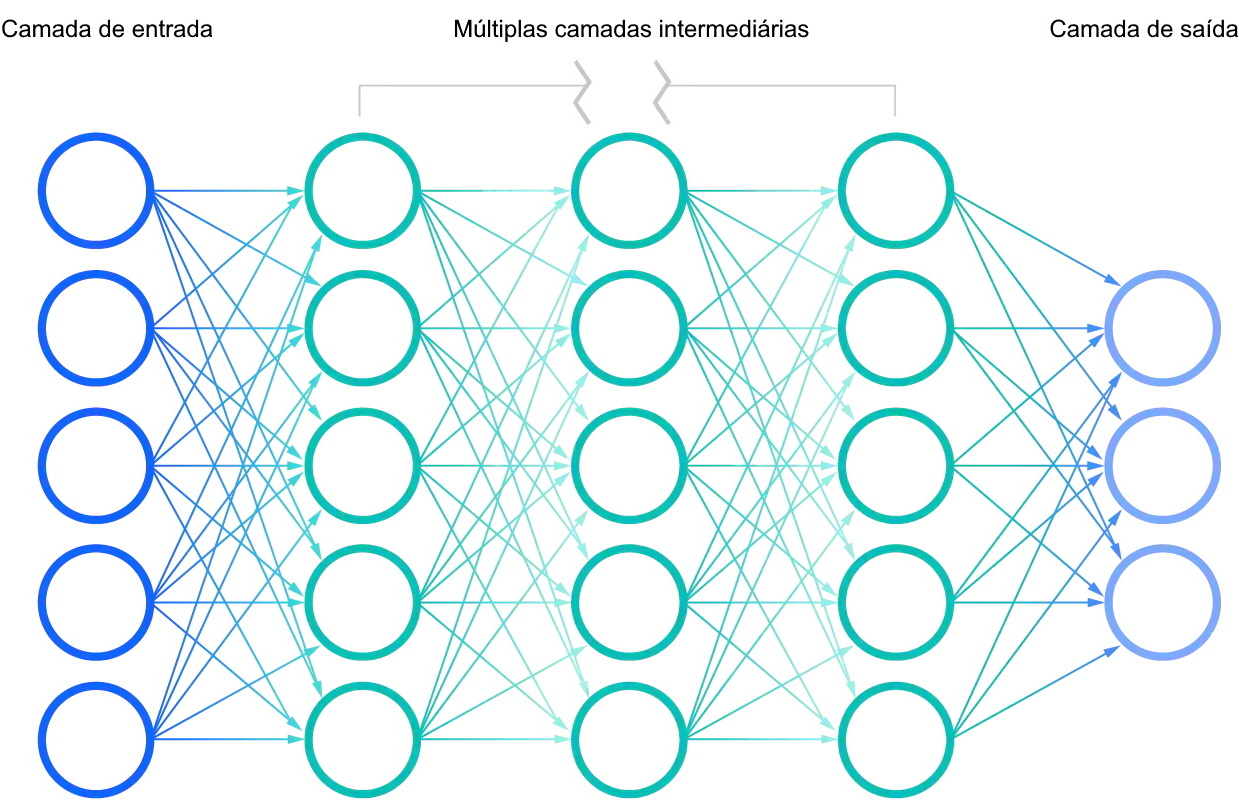
\includegraphics[width=1.0\linewidth]{images/dnn.jpg}
    \label{fig:dnn}
    \fdireta{ibm2020NN}
\end{figure}

Na \autoref{fig:dnn}, cada neurônio é representado por um círculo. 
Durante a criação da rede neural, é designado um peso, bias e função de ativação para cada neurônio. 
Durante o funcionamento, os neurônios enviam informações da esquerda para a direita. No caminho da mensagem, é realizado o cálculo da ativação com base nos seus valores para determinar se é vantajoso ou não que o próximo neurônio receba essa informação \cite{Haykin1998}.

As redes neurais são ótimas ferramentas, mas que precisam passar por um período de treinamento, onde elas aprendem quais são os pesos e limiares de cada conexão para que se tenha o resultado que se espera.
Essa etapa é onde acontece o maior custo computacional por conta da abundante quantidade de cálculos necessários, que aumentam exponencialmente pela quantidade de camadas \cite{lecun2015deep}.

\subsection{Função de ativação}

A função de ativação é um componente fundamental dos neurônios artificiais presentes nas redes neurais. 
É por meio dessa função que os neurônios decidem se devem ou não enviar um sinal para os neurônios da camada seguinte, com base na soma ponderada das entradas recebidas \cite{Goodfellow2016}.  

Em seu livro, \citeonline{haykin2009neural} explica que a função de ativação é responsável por introduzir não-linearidade nas saídas das camadas da rede, permitindo que a rede possa aprender relações não-lineares complexas entre as entradas e as saídas desejadas.
Sem a função de ativação, a rede neural seria uma sequência de operações lineares, o que diminuiria a capacidade de generalização da rede neural e prejudicaria seu desempenho em problemas mais complexos.
Concluindo, a introdução de não-linearidade pela função de ativação permite que a rede neural possa aprender e representar relações não-lineares complexas entre as entradas e as saídas desejadas.

\citeonline{haykin2009neural} ainda explica que a escolha da função de ativação a ser usada depende do tipo de problema e da arquitetura da rede neural. 
Ele destaca que as funções de ativação devem ser escolhidas de modo a permitir que a rede neural alcance o melhor desempenho possível para o problema em questão.

Existem diversas funções de ativação comumente utilizadas em redes neurais. 
Algumas das mais populares são a função sigmóide, a função \sigla{ReLU}{rectified linear unit}, a função \sigla{Tanh}{tangente hiperbólica} tanh e a função \textit{Softmax}.
Outras mais antigas mas que ainda tem utilidade são a função binária e Linear.

A função de ativação binária é uma função de ativação que transforma qualquer valor de entrada (\textit{x}) em uma saída binária, que pode ser apenas 0 ou 1. 
Essa função é frequentemente usada em redes neurais para problemas de classificação binária, onde o objetivo é separar as entradas em duas categorias distintas. Matematicamente, a função de ativação binária é definida na \autoref{eqn:limiar}.
Nessa função, se o valor da entrada \textit{x} e for maior que zero, a saída será 1. 
Caso contrário, a saída será 0.
Embora a função de ativação binária seja simples e eficiente, ela tem algumas limitações. 
Uma das principais limitações é que a função não é diferenciável em x = 0, o que torna difícil a utilização do algoritmo de \textit{backpropagation} para ajustar os pesos da rede neural durante o treinamento. 
Além disso, a função de ativação binária pode ser sensível a ruídos nos dados de entrada, o que pode prejudicar a capacidade da rede neural de generalizar para novos dados.
Por esses motivos, a função de ativação binária é geralmente substituída por funções de ativação mais adequadas para problemas mais complexos

\begin{equation}
\label{eqn:limiar}
    f(x) = \left\{\begin{matrix}
    1 & , x\geq 0\\ 
    0 & , x< 0
    \end{matrix}\right.
\end{equation}


A função de ativação linear é uma função simples que recebe uma entrada e retorna a entrada multiplicada por um peso (\textit{w}) mais um viés (\textit{b}). Matematicamente, ela é definida em \autoref{eqn:linear}. 
Essa função não é muito utilizada em redes neurais profundas, pois sua simplicidade pode levar a problemas de convergência e limitar a capacidade de aprendizado da rede. 
No entanto, ela pode ser útil em algumas situações, como em camadas de saída de redes que precisam produzir valores contínuos e não limitados.

\begin{equation}
\label{eqn:linear}
    f(x) = wx + b
\end{equation}

A função sigmóide é uma função de ativação não-linear comum em redes neurais artificiais. 
Ela tem uma curva em forma de 'S' e mapeia uma entrada (\textit{x}) para uma saída entre 0 e 1, o que é útil para representar probabilidades. 
A equação matemática para a função sigmóide é descrita na \autoref{eqn:sig}.
A função sigmóide é usada principalmente em redes neurais com uma única camada oculta, onde pode ajudar a modelar relações não-lineares entre as variáveis de entrada e saída. 
No entanto, ela tem algumas limitações, como o problema de desvanecimento de gradiente, que pode dificultar o treinamento de redes neurais mais profundas.

    \begin{equation}
    \label{eqn:sig}
    \sigma(x) = \frac{1} {1 + e^{-x}}
    \end{equation}

A função Tanh (\autoref{eqn:tanh}) é uma versão escalonada da função sigmóide (\autoref{eqn:tanhsig}), que busca solucionar os problemas que a função sigmóide possui.
Assim como a função sigmóide, a função Tanh é não linear e possui uma forma de 'S', mas com valores de saída variando de -1 a 1 em vez de 0 a 1, dessa forma possuindo simetria e tanto valores positivos quanto negativos.
Além disso, a função Tanh é simétrica e tem uma região plana em torno de 0, o que significa que, para valores de entrada (\textit{x}) próximos de 0, a função retorna valores próximos de 0.
No entanto, a função Tanh também pode ser propensa a problemas de gradiente desvanecente em redes neurais profundas.
    
\begin{equation}
\label{eqn:tanh}
Tanh(x) = \frac{e^x - e^{-x}}{e^x + e^{-x}} = \frac{1 - e^{-2x}}{1 + e^{-2x}}
\end{equation}

\begin{equation}
\label{eqn:tanhsig}
Tanh(x) = 2\sigma(2x) - 1
\end{equation}

A função de ativação ReLU (\autoref{eqn:relu}) é uma função matemática que transforma um valor de entrada em um valor não negativo.
A função ReLU é uma função não linear e é frequentemente usada como função de ativação em redes neurais artificiais, especialmente em camadas ocultas. 
A principal vantagem da função ReLU é que ela é computacionalmente eficiente e fácil de calcular.

A função ReLU tem uma região plana para valores de entrada (\textit{x}) negativos, onde a função retorna 0. 
Para valores de entrada positivos, a função retorna o próprio valor de entrada. 
A função ReLU é, portanto, uma função de ativação não saturante, o que significa que ela não tem um limite superior no valor de saída. 
Isso pode ser útil para problemas com saídas muito grandes, como detecção de objetos em imagens.
No entanto, a função ReLU pode levar a problemas de "neurônios mortos" em que o neurônio não é ativado para nenhum valor de entrada, resultando em uma rede neural com menos capacidade de aprendizado. 
Para lidar com esse problema, foram propostas variações da função ReLU, como a função \textit{Leaky} ReLU e a função \sigla{ELU}{Exponential Linear Unit}.


\begin{equation}
\label{eqn:relu}
Relu(x) = max(0, x)
\end{equation}

A função de ativação \textit{Softmax} é uma função matemática que transforma um vetor de valores em uma distribuição de probabilidade. 
A função é definida em \autoref{eqn:softmax}, onde onde $x_{i}$ é o i-ésimo valor de entrada e $K$ é a quantidade de valores de entrada.
Dessa forma, a soma é calculada sobre todos os valores de entrada.

\begin{equation}
\label{eqn:softmax}
\sigma(x_i) = \frac{e^{x_{i}}}{\sum_{j=1}^K e^{x_{j}}} \ \ \ for\ i=1,2,\dots,K
\end{equation}

A função \textit{Softmax} é uma função não linear e é frequentemente usada como função de ativação na camada de saída de uma rede neural classificadora. 
A função \textit{Softmax} é usada para transformar as saídas da rede neural em uma distribuição de probabilidade sobre as classes possíveis. 
Cada saída da rede neural é transformada em um valor entre 0 e 1, de modo que a soma de todas as saídas seja igual a 1.

A função \textit{Softmax} é especialmente útil em problemas de classificação multiclasse, onde a rede neural precisa classificar uma entrada em várias classes possíveis. 
A função \textit{Softmax} fornece uma saída normalizada que pode ser interpretada como uma probabilidade de pertencer a cada classe.
No entanto, a função \textit{Softmax} pode ser sensível a valores muito grandes ou muito pequenos de entrada, o que pode levar a problemas de estabilidade numérica. 
Além disso, a função \textit{Softmax} assume que as classes são mutuamente exclusivas e não pode lidar com casos em que uma entrada pode pertencer a mais de uma classe.


\subsection{Feed-forward e Backward propagation}

A propagação feed-forward, ou propagação direta, é um dos principais algoritmos utilizados em redes neurais artificiais para realizar o processamento de dados. 
De forma geral, esse algoritmo consiste em propagar os sinais de entrada da camada anterior para a próxima camada da rede neural, até que o sinal de saída seja obtido na camada de saída. 
Durante essa propagação, os pesos sinápticos são atualizados em cada camada, utilizando um método de otimização, como o gradiente descendente.

Assim como a \autoref{fig:ffp} exemplifica, as entradas %($x_{1}, x_{2}, ..., x_{m}$) 
são processadas pelas primeiras camadas de neurônios % ($\omega_{1}, \omega_{2}, ..., \omega_{m}$)
, que aplicam uma função de ativação na soma dos resultados dos neurônios, para produzir uma saída que é passada para a próxima camada. 
Esse processo é repetido até que a saída final seja produzida pela última camada de neurônios. 
Esse tipo de rede neural é chamado de '\textit{feed-forward}' porque as informações fluem em uma única direção, da entrada para a saída, sem ciclos ou realimentação \cite{Goodfellow2016}.

\begin{figure}[htb]
    \centering
    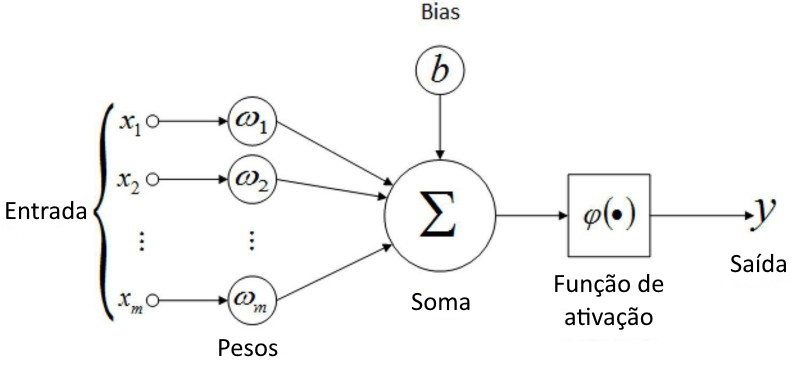
\includegraphics[width=1\linewidth]{TCC UFG/images/aannbias.jpeg}
    \caption{Propagação Feed-Foward.}
    \label{fig:ffp}
    \fadaptada{haykin2009neural}
\end{figure}

De acordo com \citeonline{Goodfellow2016}, a propagação \textit{feed-forward} é a base para muitas arquiteturas de redes neurais, como redes neurais de camadas densas, redes convolucionais e redes recorrentes. 
Além disso, esse algoritmo tem sido amplamente utilizado em várias aplicações de aprendizado de máquina, como reconhecimento de fala, processamento de linguagem natural, classificação de imagens e previsão de séries temporais.

Para realizar a propagação \textit{feed-forward}, é necessário definir a arquitetura da rede neural, que inclui o número de camadas, o número de neurônios em cada camada e a função de ativação utilizada em cada neurônio. 
Segundo \citeonline{Rumelhart1986}, a escolha adequada da arquitetura é crucial para garantir a eficiência e a precisão da rede neural.

Por fim, a propagação \textit{feed-forward} é um processo iterativo e computacionalmente intenso, que pode levar a problemas de convergência lenta ou instável. 
Para contornar esses problemas, vários métodos de regularização, como \textit{dropout} e \textit{L2 regularization}, foram desenvolvidos para melhorar a generalização da rede neural \cite{srivastava2014}.

Propagação para trás, ou \textit{Backward Propagation}, comumente chamado de \textit{backpropagation} é o método de treinamento de redes neurais mais utilizado, podendo ser considerado a essência do treinamento das redes neurais atuais \cite{builtinML}.

O \textit{backpropagation} é um algoritmo de aprendizado de rede neural que funciona de forma contrária ao \textit{feedforward propagation}. 
Enquanto o \textit{feedforward propagation} processa a entrada da rede neural camada por camada, produzindo uma saída, o \textit{backpropagation} começa com a saída da rede e retrocede pelos seus pesos, atualizando-os de acordo com a sua contribuição para o erro da rede \cite{Rumelhart1986}.

O processo de retropropagação é iniciado após o cálculo da saída da rede neural para uma determinada entrada. A partir daí, o gradiente da função de erro é calculado em relação aos pesos da rede. 
Esse gradiente representa a sensibilidade da função de erro em relação a cada peso da rede neural.

Em seguida, o gradiente é propagado de volta pela rede neural, camada por camada, usando a regra da cadeia. 
Em cada camada, o gradiente é usado para calcular a contribuição dos pesos para o erro da rede, permitindo que eles sejam ajustados de acordo com essa contribuição. 
Esse processo é repetido várias vezes até que a rede neural atinja um nível satisfatório de desempenho \cite{Goodfellow2016}.

Em resumo, enquanto o \textit{feedforward propagation} processa a entrada da rede neural e produz uma saída, o \textit{backpropagation} retrocede pelos pesos da rede neural para atualizá-los de acordo com a sua contribuição para o erro da rede.
Essa técnica de aprendizado supervisionado é fundamental para treinar redes neurais profundas e tem sido usada com sucesso em diversas aplicações de aprendizado de máquina \cite{Goodfellow2016}.

\subsection{Sobreajuste e métodos de regularização}

O sobreajuste, ou \textit{overfitting}, é um problema comum em modelos de aprendizado de máquina. 
Ele ocorre quando um modelo é muito complexo, ou profundo no caso das redes neurais convolucionais, e se ajusta muito bem aos dados de treinamento, mas apresenta um desempenho ruim em novos dados. 
Esse problema pode ser evitado com o uso de métodos de regularização.

Existem diferentes métodos de regularização, e um dos mais comuns é o \textit{dropout}. 
A técnica do \textit{dropout} consiste em desativar aleatoriamente alguns neurônios da rede neural durante o treinamento, de modo que a rede seja forçada a aprender a redundância dos dados \cite{srivastava2014}. 
Outra técnica de regularização é a regularização L1 e L2, que adiciona termos de penalidade aos pesos da rede durante o treinamento. 
A regularização L1 adiciona uma penalidade proporcional à soma dos valores absolutos dos pesos, enquanto a regularização L2 adiciona uma penalidade proporcional à soma dos quadrados dos pesos \cite{lecun1998gradient}.

Vale citar que para a redução do \textit{overfitting}, também é necessário que aconteça a escolha adequada de hiperparâmetros, como o tamanho dos lotes ou \textit{batchs}, o número de épocas e a taxa de aprendizado.
Por fim, técnicas de avaliação de desempenho, como validação cruzada e conjunto de validação podem ajudar a identificar e prevenir o \textit{overfitting} \cite{shortImageDeep}.

\subsection{Transferência de aprendizado}

De acordo com \citeonline{Bengio2016}, a transferência de aprendizado se refere à utilização do aprendizado realizado em um contexto de forma a melhorar de forma geral o aprendizado em outro contexto.
Logo, a transferência de aprendizado é uma metodologia para otimização que permite acelerar o processo de aprendizagem e aumentar a performance dos resultados.

Ainda segundo \citeonline{Bengio2016}, na transferência de aprendizado, primeiramente ocorre o treinamento de uma rede neural em uma determinada base de dados para realizar uma tarefa para que então se possa reaproveitar, ou transferir as características aprendidas para uma segunda rede neural que aprende em alguma base da dados para alguma tarefa. 
Esse procedimento tende a funcionar quando as características aprendidas inicialmente são generalizadas ou semelhantes às da outra base de dados.

Esse processo se tornou popular no campo de \textit{deep learning} por diminuir o custo computacional de treinamento, onde há geralmente apenas um pequeno treinamento para aperfeiçoar o modelo pré-treinado para a tarefa determinada, o que requer menor quantidade de dados também \cite{builtintl}. 
De forma prática, essa transferência é tido como a passagem dos pesos de um modelo para outro \cite{builtintl}. 


\section{Redes neurais convolucionais}

\sigla{CNN}{\textit{Convolutional Neural Network}} são uma subclasse de redes neurais profundas, usadas principalmente para análise de conteúdo visual \cite{valueva2020application}. 
A diferença das CNNs em relação a outras redes neurais é que elas não usam o modelo padrão de neurônios independentes uns dos outros, isso acontece pois imagens são matrizes de pixels próximos tendem a se complementar em sentido. 
Para lidar com essa dependência, as CNNs utilizam filtros ou \textit{kernels}, que permitem que a rede aprenda a identificar padrões espaciais em imagens e até temporais em vídeos \cite{lecun1998gradient}.

\begin{figure}[htb]
    \centering
    \caption{Representação genérica de CNN para classificação.}
    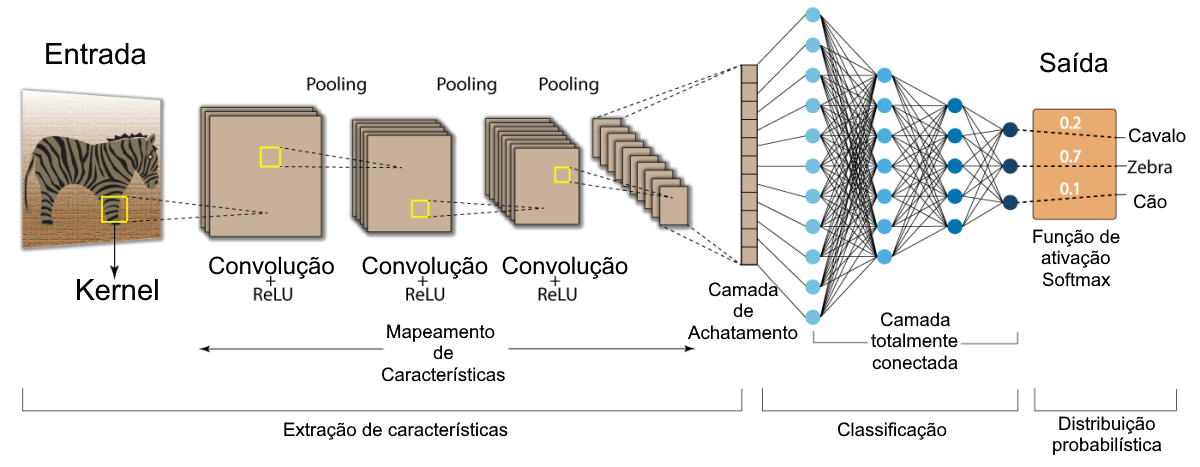
\includegraphics[width=1.0\linewidth]{TCC UFG/images/cnn_example.png}
    \label{fig:genconv}
    \fadaptada{imagemZebra}
\end{figure}

As redes neurais convolucionais são geralmente arquitetadas em blocos. 
Cada bloco é composto por uma ou mais camadas convolucionais, seguidas por camadas de \textit{pooling} e, possivelmente, camadas de normalização. 
Esses blocos são organizados em uma hierarquia, permitindo que a rede neural aprenda gradualmente características cada vez mais complexas. 
A arquitetura em blocos também permite que a rede neural seja projetada de forma modular, permitindo que diferentes arquiteturas sejam criadas a partir de combinações de blocos \cite{simonyan2014very}. 
Alguns exemplos de arquiteturas em blocos amplamente utilizadas em redes neurais convolucionais incluem a VGG, ResNet e Inception.


\subsection{Camada de convolução}

Imagens são estruturas de dados gigantescas, sendo matrizes que guardam até 9 milhões de pixels em uma imagem 4K. 
Logo, as CNNs buscam reduzir essas imagens em uma forma mais fácil de processar sem perder os atributos ou características importantes da imagem \cite{sumitCNN}. 
O processo responsável por essa diminuição é o processo de convolução através de filtros.

A camada de convolução, como o nome já sugere, aplica uma operação de convolução entre os pesos da camada e os dados de entrada para produzir um mapa de características.
Durante a convolução, uma janela deslizante é usada para percorrer toda a imagem de entrada. 
Em cada posição da janela, é feita uma multiplicação elemento a elemento entre os valores da janela e os pesos da camada. 
Em seguida, o resultado dessas multiplicações é somado para produzir um único valor de saída. 
Esse processo é repetido para todas as posições da janela, produzindo um mapa de características.
Esse processo pode ser visualizado na \autoref{fig:conv}.

\begin{figure}[htb]
    \centering
    \caption{Exemplo de convolução.}
    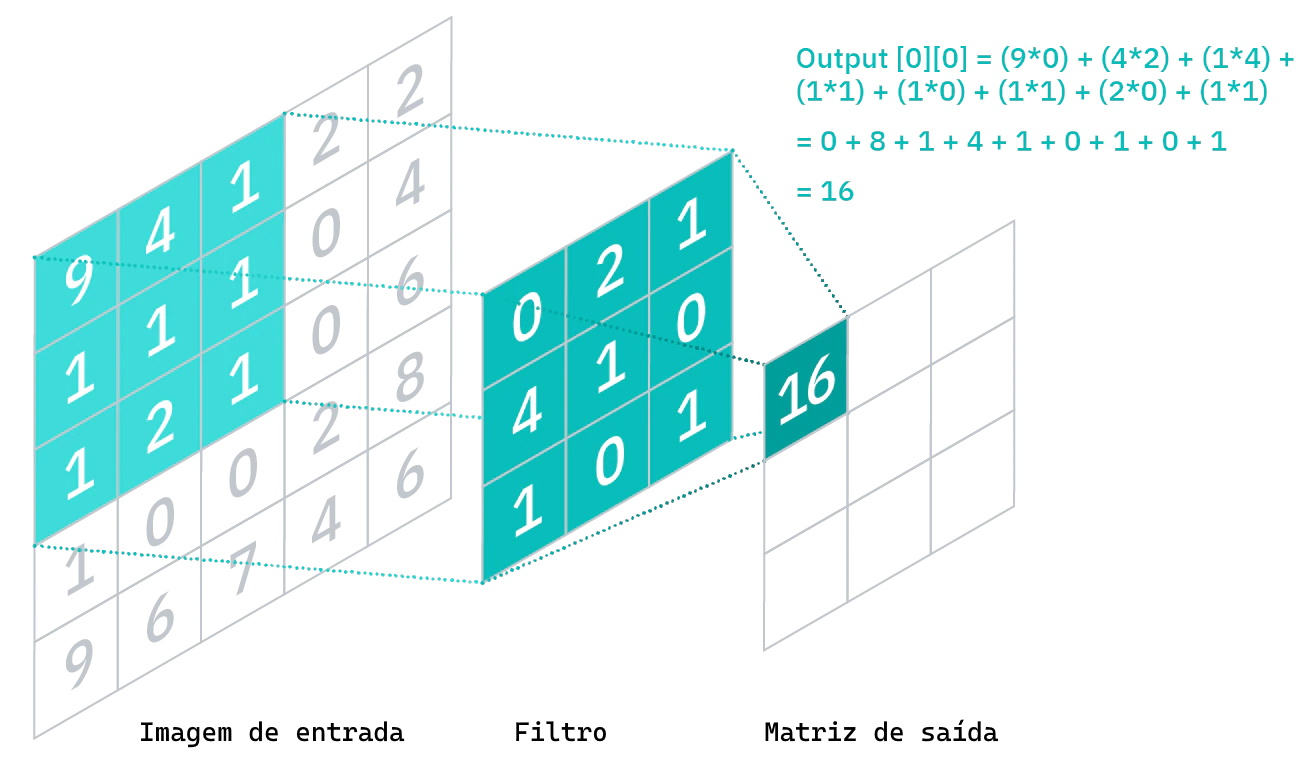
\includegraphics[width=0.8\linewidth]{TCC UFG/images/conv.jpg}
    \label{fig:conv}
    \fadaptada{ibm2020CNN}
\end{figure}

O tamanho da janela é controlado por um parâmetro chamado tamanho do filtro. 
O número de filtros é outro parâmetro que controla quantas características diferentes são extraídas da imagem. 
Cada filtro produz um mapa de características, que é combinado para formar o mapa de características da camada.

Além disso, a camada de convolução pode apresentar outras operações como \textit{padding} e \textit{stride}. 
O \textit{padding} é usado para adicionar uma borda de zeros à imagem de entrada para manter o tamanho do mapa de características de saída. 
O \textit{stride} controla o quanto a janela desliza pela imagem de entrada em cada etapa.


\subsection{Camada de pooling}

A camada de \textit{pooling} é utilizada principalmente para reduzir a dimensionalidade do mapa de características gerado pela camada de convolução, reduzindo o número de parâmetros da rede e evitando o \textit{overfitting} \cite{lecun1998gradient}.
Via de regra, essa camada é aplicada após a camada de convolução, geralmente reduzindo a dimensão espacial do mapa de características e mantendo apenas as características mais importantes. 

Normalmente, são utilizados dois tipos de \textit{pooling}: \textit{max pooling} e \textit{average pooling}.
O mais comum é o \textit{max pooling}, que extrai o valor máximo de cada região do mapa de características.
Já o \textit{average pooling}, extrai a média da região do mapa de características \cite{sumitCNN}.


No entanto, as camadas de \textit{pooling} também podem ter algumas desvantagens, como a perda de informações espaciais e a introdução de distorções na imagem de entrada. 
Essas desvantagens podem ser minimizadas por meio da escolha adequada do tamanho do filtro e do \textit{stride}.

Vale ressaltar que, embora a camada de convolução e a camada de \textit{pooling} tenham o efeito de reduzir a resolução espacial do mapa de características de entrada, elas têm propósitos diferentes na rede neural convolucional.
A camada de convolução tem o objetivo de extrair características e tem como resultado um mapa de características, e nisso como consequência acontece a diminuição da resolução caso não configurado para que não o faça.
Enquanto a camada de \textit{pooling} tem como objetivo principal reduzir a resolução espacial do mapa de características \cite{divaSeg}.

\subsection{Camada de achatamento}

A camada de achatamento tem como função transformar o mapa de características gerado pelas camadas convolucionais em um vetor unidimensional, que pode ser processado pelas camadas totalmente conectadas, ou densas, da rede neural.
Por conta disso, essa camada é geralmente adicionada ao final das camadas convolucionais e antes das camadas densas \cite{lecun2015deep}.

A camada de achatamento é importante porque as camadas densas ou totalmente conectadas requerem uma entrada de vetor unidimensional, enquanto as camadas convolucionais geralmente trabalham com entradas em forma de matriz ou tensor. 
E embora não seja seu foco, a camada de achatamento reduz o número de parâmetros da rede, o que pode ajudar a evitar o \textit{overfitting} e a acelerar o treinamento \cite{lecun2015deep}.


\subsection{Camada totalmente conectada}

Em uma camada totalmente conectada, ou densa, todos os neurônios estão conectados com todos os neurônios da camada anterior. 
Isso significa que cada neurônio de entrada é conectado a cada neurônio de saída. 
Essa conexão densa permite que a camada aprenda representações complexas dos dados e forneça uma saída mais precisa.
Essas camadas geralmente estão localizadas no final da rede neural, depois de uma série de camadas de convolução e de \textit{pooling} \cite{lecun2015deep}. 

Usualmente, a camada densa é utilizada como um classificador, que recebe as características extraídas pelas camadas anteriores e realiza uma classificação ou regressão final \cite{sumitCNN}.
Esse comportamento pode ser visualizado na \autoref{fig:dnn}, onde cada neurônio está ligado a todos os neurônios da próxima camada.

\subsection{Arquiteturas}
\label{dl:arquiteturas}

As arquiteturas em redes neurais convolucionais são as estruturas que determinam como as camadas dessas redes serão organizadas, incluindo o número de camadas, o tipo de camadas, o número de filtros, entre outros aspectos \cite{lecun1998gradient}.

A seguir, são apresentadas algumas das arquiteturas mais conhecidas.

\subsubsection{Arquitetura AlexNet}

% Contextualização do modelo AlexNEt
AlexNet  \cite{alexnetAnalyticsVidhya2021} é uma arquitetura premiada pela competição \textit{ImageNet} de 2012, popularizando a utilização de camadas de convolução cada vez mais profundas, uma de suas principais características, que o tornava um modelo com ótimas performances ao ônus de um considerável aumento no custo computacional \cite{krizhevsky2017imagenet}. 
O modelo conta com oito camadas com cerca de 63 milhões de parâmetros com capacidade de aprendizado, separados em cinco camadas de convolução e três camadas totalmente conectadas onde são utilizados \textit{pooling} e \textit{dropout}, nas saídas de suas camadas é utilizado a função de ativação Relu, exceto na saída final, onde se utiliza da função de ativação \textit{Softmax} \cite{alexnetAnalyticsVidhya2021}. 

A arquitetura AlexNet pode ser vista na \autoref{fig:alexnet}.

\begin{figure}[htb]
    \centering
    \caption{Arquitetura AlexNet.}
    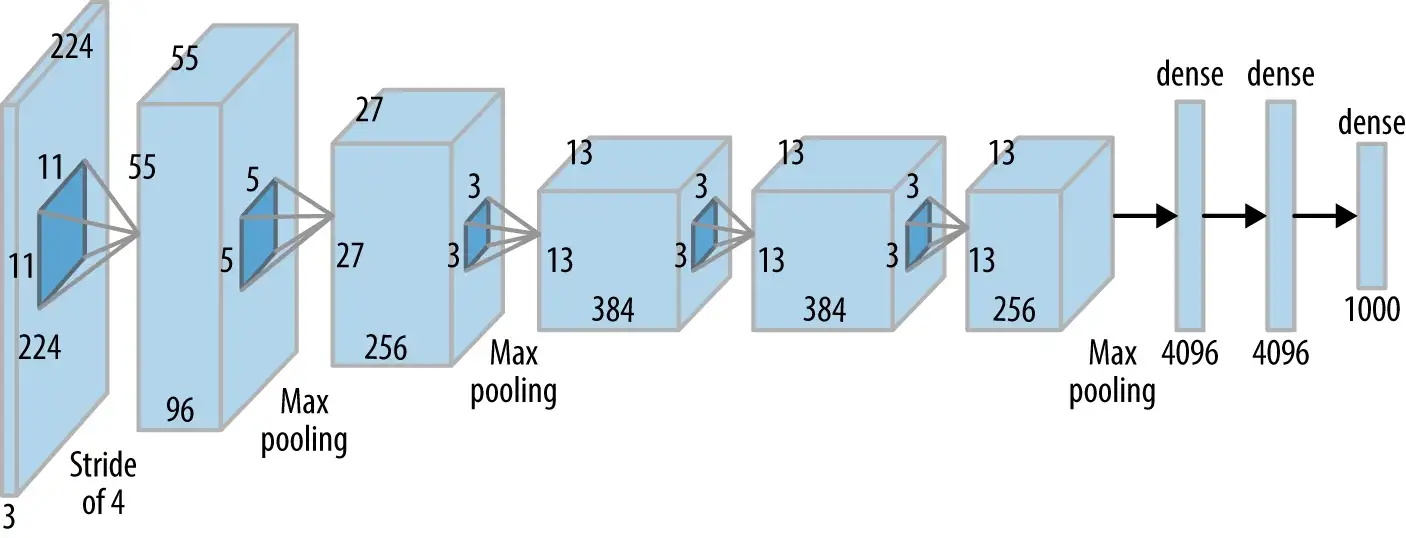
\includegraphics[width=1\linewidth]{images/alexnet.jpg}
    \label{fig:alexnet}
    \fdireta{aqeel2019}
\end{figure}


\subsubsection{Arquitetura VGG}
% Contextualização do modelo VGG16
O grupo de pesquisa \textit{Visual Geometry Group} (VGG) \cite{simonyan2014very}, foi com seus modelo VGG 16 vencedor na modalidade de classificação com localização no desafio \textit{ImageNet} de 2014 e tendo uma boa colocação na de apenas classificação, onde alcançou 92,7\% no teste de acurácia entre a base de dados do \textit{ImageNet}, constituída por 14 milhões de imagens divididas em 1000 classes \cite{ILSVRC15}. 
A principal ideia proposta pelo grupo é a de usar filtros de convolução muito menores, matrizes de tamanho 3x3 com o deslocamento de apenas um pixel por toda a rede neural, sendo bem menor que outros modelos padrões da época como AlexNet \cite{krizhevsky2017imagenet}, que utiliza matriz de convolução de tamanho 11x11 com deslocamento de 4 pixels.
O funcionamento de tal ideia é de utilizar mais camadas para compensar o menor tamanho do filtro, já que no final de cada camada há uma função de ativação, há uma maior utilização de tal processo, fazendo com que a rede se torne mais discriminante  e resultando também no aumento da convergência da rede.
No que diz respeito ao custo computacional, mesmo com aumento na quantidade de camadas, a matriz 3x3 requer menos parâmetros no geral, logo, requer menor potência computacional \cite{GreatLearningVgg16}.


A principal característica do modelo VGG é sua profundidade, com 16 ou 19 camadas convolucionais, que fazem com que o modelo tenha um grande número de parâmetros treináveis. 
Outra particularidade do VGG é que todas as camadas convolucionais têm um filtro 3x3 com o objetivo de reduzir o número de parâmetros e aumentar a capacidade de representação da rede. 
O VGG também utiliza camadas de \textit{max pooling} com filtros de 2x2 para reduzir a resolução espacial das características. 
Além disso, o modelo utiliza camadas densas no final da arquitetura para realizar a classificação final. 
Por causa de sua profundidade e alta capacidade de representação, o modelo VGG alcançou altas performances em diversos conjuntos de dados de imagens, como o \textit{ImageNet} \cite{simonyan2014very}.

Em específico, a VGG16 é constituída por dois blocos iniciais, cada um com duas camadas de convolução seguida pela camada de \textit{max-pooling}, em seguida três blocos intermediários, cada um com três camadas de convolução seguida pela camada de \textit{max-pooling} e para finalizar três camadas densas de convolução.
A arquitetura VGG, em específico o modelo VGG16, pode ser vista na \autoref{fig:vgg16}.

\begin{figure}[htb]
    \centering
    \caption{Configuração do modelo VGG16.}
    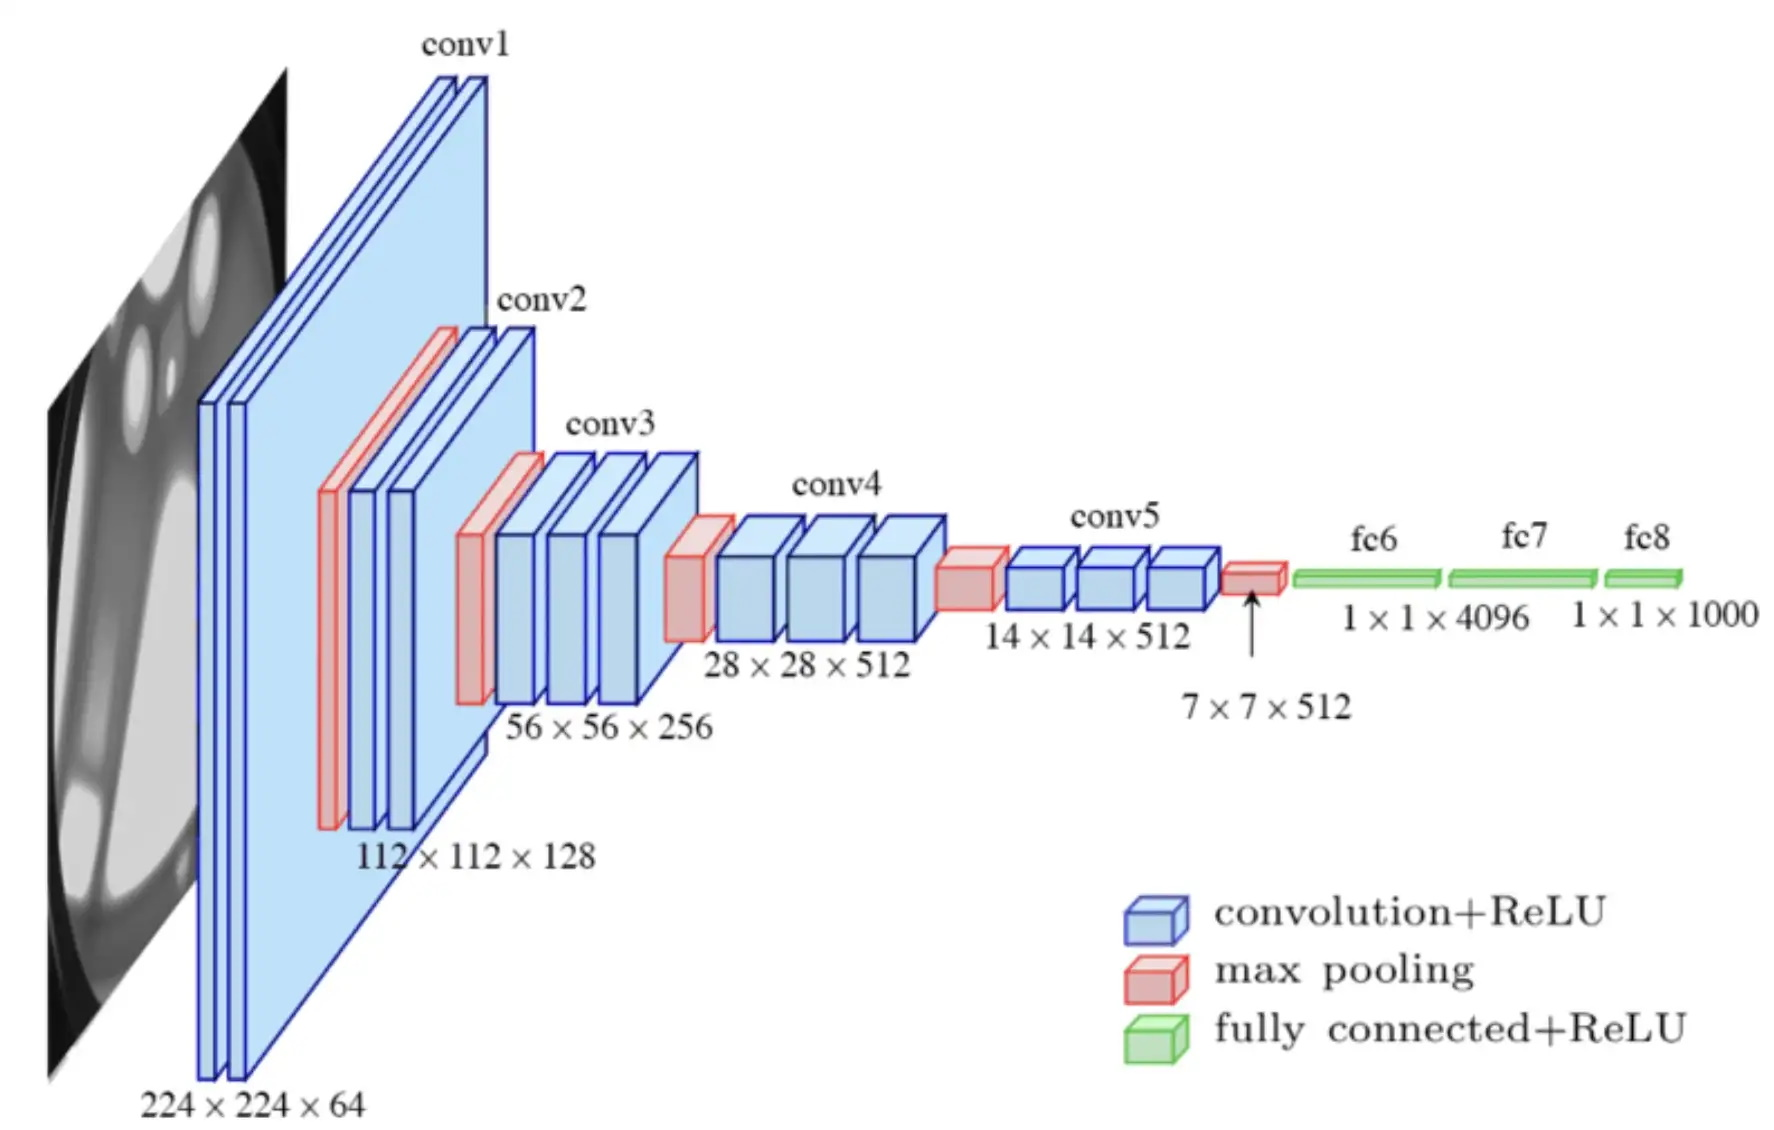
\includegraphics[width=0.8\linewidth]{images/vgg16.jpg}
    \label{fig:vgg16}
    \fdireta{khuyen2021}
\end{figure}



\subsubsection{Arquitetura DenseNet}

% Contextualização do modelo DenseNet
Redes convolucionais densamente conectadas, ou arquitetura DenseNet \cite{huang2017densely} é um modelo recente que promete ser o próximo passo no que diz respeito em aumentar a profundidade das redes convolucionais \cite{PabloDenseNet2018}. 
Após a popularização do aumento da profundidade das camadas convolucionais por conta do modelo AlexNet \cite{krizhevsky2017imagenet} em 2012, houve um constante aumento na profundidade de diversos modelos chegando em números massivos, porém esse aumento no caminho que a informação precisa percorrer desde a camada inicial até a camada final se tornou tão grande que o dado pode ser deturpado e não se tornar nada \cite{PabloDenseNet2018}, além do custo computacional exorbitante. 
Para contornar tais problemas, o DensetNet busca simplificar o modelo de conectividade entre as camadas enquanto garanta que o fluxo de informações não seja perturbado, dessa forma foi utilizado um modelo de reutilização dos extratores de características, realizando conexões que ligam todas camadas diretamente com todas as outras \cite{huang2017densely}. 
Por conta disso o modelo DenseNet precisa de menos parâmetros e elimina a necessidade de camadas redundantes. Se comparado com classificador de uma rede neural genérica que depende dos resultados da última camada de rede, o DenseNet consegue utilizar de forma mais inteligente os resultados já produzidos, obtendo um resultado melhor em performance e precisão.
A \autoref{fig:densenet} ilustra a arquitetura padrão do modelo.

\begin{figure}[htb]
    \centering
    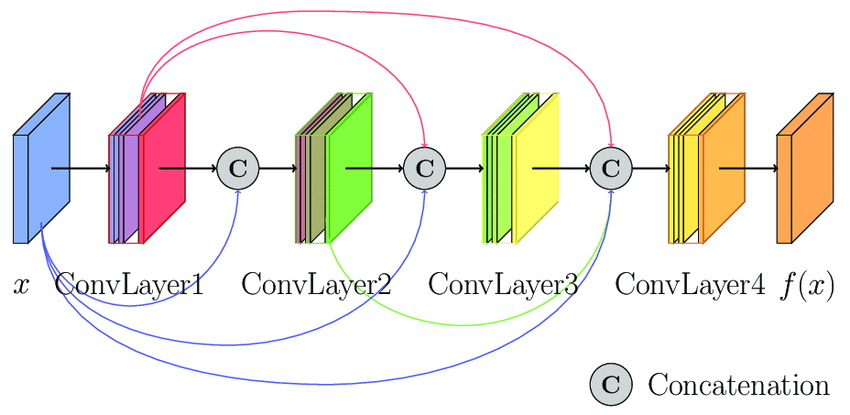
\includegraphics[width=0.8\linewidth]{images/densenet.jpg}
    \caption{Exemplo dos blocos densos em uma DenseNet.}
    \label{fig:densenet}
    \fdireta{mazza2019}
\end{figure}



\subsubsection{Arquitetura Inception V3}
% Contextualização do modelo Inception V3

O modelo \textit{Inception V3}  é uma rede neural convolucional profunda, desenvolvida pela equipe do Google em 2015 \cite{szegedy2015going}. 
O objetivo do modelo é alcançar alta acurácia em tarefas de classificação de imagens, utilizando uma arquitetura que reduz a quantidade de parâmetros e, ao mesmo tempo, mantém um alto desempenho.

Uma das principais características do \textit{Inception V3} é a utilização do módulo de convolução \textit{Inception}, que utiliza diferentes tamanhos de filtros (1x1, 3x3 e 5x5) em paralelo para extrair diferentes características das imagens. 
Além disso, o modelo também utiliza uma camada de \textit{pooling} antes do módulo \textit{Inception} para reduzir a resolução espacial do mapa de características de entrada \cite{szegedy2015going}.

O \textit{Inception V3} também utiliza técnicas de regularização, como o \textit{dropout} e a normalização por lote, para prevenir o \textit{overfitting} durante o treinamento da rede.
O modelo \textit{Inception V3} é um dos modelos mais populares em aplicações de visão computacional, tendo sido utilizado em diversas competições de classificação de imagens, como o \sigla{ILSVRC}{\textit{ImageNet Large Scale Visual Recognition Challenge}} em 2015 e 2016.
O modelo de arquitetura do \textit{Inception V3} pode ser visualizado na  \autoref{fig:inceptionv3}.

\begin{figure}[htb]
    \centering
    \caption{Modelo de arquitetura do Inception V3.}
    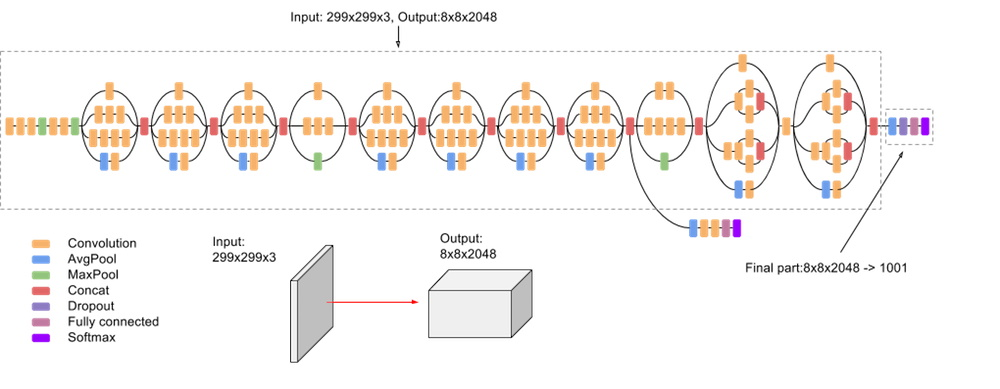
\includegraphics[width=1\linewidth]{images/inceptionv3.jpg}
    \label{fig:inceptionv3}
    \fdireta{googleCloudInceptionv3}
\end{figure}



\subsubsection{Arquitetura ResNet}
% Contextualização do modelo ResNet
\sigla{ResNet}{\textit{Residual neural network}} é uma rede neural convolucional cuja principal característica é ter uma profundidade muito maior que os outros modelos, variando desde 30 camadas até a casa dos milhares \cite{he2016deep}.
A arquitetura ResNET venceu o campeonato \textit{ImageNet} 2015 \cite{deng2009imagenet}, e desde então vem sido o modelo computacional com mais citações \cite{schmidhubermost}. 
Os modelos mais conhecidos desse modelo são ResNet-34, ResNet-50, and ResNet-101 tendo esses nomes por terem profundidade de 34, 50 e 101 respectivamente.

 O principal desafio ao treinar redes profundas é o problema de desvanecimento do gradiente, que ocorre quando o gradiente se torna tão pequeno que a rede não consegue aprender com as atualizações de peso. 
 O ResNet resolve esse problema introduzindo conexões residuais entre as camadas da rede, permitindo que a informação de entrada flua diretamente para camadas posteriores \cite{Vanshika2021}.
 Esse processo pode ser observado na \autoref{fig:camada_residual}, onde a entrada \textit{x} flui diretamente para uma camada posterior.

Teoricamente, a utilização das conexões residuais faz com que os parâmetros aprendidos sejam guardados e repassados para as camadas futuras, dessa forma, mesmo que aconteça os problemas como a dissipação de gradiente, haverá uma camada posterior que receberá de volta os parâmetros aprendidos \cite{Vanshika2021}. 
O agrupamento dessas camadas, desde onde há o começo de um atalho, até a camada conectada por este atalho é chamado de bloco residual \cite{he2016deep}.
O bloco em questão é composto por duas camadas convolucionais, seguidas por uma operação de adição que permite que a ativação da camada anterior seja adicionada à ativação atual. 
Essa operação de adição permite que a rede aprenda apenas as diferenças entre a ativação atual e a ativação anterior, ao invés de ter que re-aprender toda a representação da entrada \cite{he2016deep}.

Por fim, o ResNet  consegue utilizar blocos residuais que contêm múltiplas camadas convolucionais em paralelo, permitindo que a rede aprenda múltiplas representações de uma mesma entrada \cite{Vanshika2021}.


\begin{figure}[htb]
    \centering
    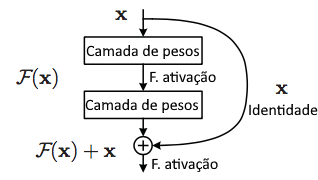
\includegraphics[width=0.5\linewidth]{TCC UFG/images/adap_cama_res.png}
    \caption{Exemplo de bloco residual.}
    \label{fig:camada_residual}
    \fadaptada{he2016deep}
\end{figure}
 


\chapter{Metodologia}
\label{chapter:metodologia}
\section{Considerações iniciais}
Neste capítulo apresenta a metodologia utilizada para execução deste trabalho, desde escolha de base de dados, montagem e escolha das arquiteturas de CNN`s, até o método de treinamento e métricas para avaliação.

\section{Base de dados}
A partir da recomendação de \citeonline{zoubir2021crack}, foram selecionados as bases de \citeonline{zhang_base2018}; \citeonline{maguire2018sdnet2018}, chamada de SDNET2018; \citeonline{zoubir2021crack} e \citeonline{xu2019automatic}.

\subsection{Obtenção e especificidades das bases}
\label{sub:bases}

As bases utilizadas foram encontradas e baixadas da Internet, a partir de seus artigos. 
Todas as bases são rotuladas para classificação, com imagens divididas em dois rótulos. 
Embora as bases usem diferentes nomes para os rótulos, elas podem ser renomeadas e reorganizadas como "positivo" para imagens com fissuras e "negativo" para imagens sem fissuras sem que altere o significado.

A base elaborada por \citeonline{zhang_base2018} é composta por um total de 40.000 imagens de resolução $227 \times 227$, as quais foram divididas em 20.000 positivas e 20.000 negativas.
As imagens foram tiradas em construções do campus \sigla{METU}{Middle East Technical University} utilizando um \textit{smartphone}, obtendo 458 imagens de alta resolução ($4032 \times 3024$).
Fora a divisão e rotulação, não acontece  nenhum processamento de \textit{data augmentation}.
Por fim, as imagens apresentam diferentes condições de iluminação e texturas.

SDNET2018 é um conjunto de dados de imagens rotuladas de uso para algoritmos de detecção de fissuras em concreto baseados em inteligência artificial \cite{maguire2018sdnet2018}.
Este conjunto contém mais de 56.000 imagens de decks de pontes, paredes e pavimentos de concreto com e sem fissuras, com fissuras tão estreitas quanto 0,06 mm e tão largas quanto 25 mm. 
Além disso, o conjunto de dados inclui imagens com várias obstruções, como sombras, aspereza superficial, escalonamento, bordas, buracos e detritos de fundo.

Seus criadores, \citeonline{maguire2018sdnet2018}, capturaram 230 imagens de superfícies de concreto trincadas e não trincadas (54 decks de pontes, 72 paredes, 104 pavimentos) usando uma câmera digital Nikon de 16 MP. 
As superfícies foram localizadas no sistema de laboratório \sigla{SMASH}{\textit{Utah State University system, material, and structural health}} e nas estradas e calçadas do campus da universidade. 
Cada imagem foi segmentada em sub-imagens de $256 \times 256$ pixels.

O artigo de \citeonline{zoubir2021crack} é o que recomenda as outras bases de dados, no entanto, a metodologia empregada consiste em utilizar uma base de dados própria do autor.
Para tal, foram coletadas 572 imagens de resolução $5152 \times 3864$ de plataformas e pilares de concreto com fissuras, sendo que para melhorar a diversidade do conjunto de dados proposto as imagens apresentam diferentes condições de iluminação e superfície como: Rugosidade, cor, umidade e luz forte. 
As imagens são então recortadas em 1304 imagens fissuradas e 5634 não fissuradas.
Porém, apenas 1.050 imagens fissuradas e 2.772 não fissuradas são disponibilizadas para \textit{download}.

Diferentes tipos e tamanhos de fissuras estão presentes nas imagens. 
Além disso, o conjunto de dados apresenta alterações de superfície desafiadoras, tais como manchas e marcas. 
É importante mencionar que algumas imagens que não possuem fissuras contêm juntas de concreto, que podem ser confundidas com fissuras durante a classificação, e ainda podem ser encontrados pequenos defeitos.

Já o artigo de \citeonline{xu2019automatic}, utiliza a base de dados proposta por \citeonline{LiLiangBase} aplicando \textit{data augmentation}.
A base original é composta por 2.068 imagens de imagens de fissuras, coletadas pela câmera \textit{Phantom 4 Pro's CMOS} com resolução de $1024 \times 1024$.

Por conta da base original possuir apenas imagens com fissuras, \citeonline{xu2019automatic} relata que foi necessário recortar as imagens originais em quatro imagens de $512 \times 512$, assim obtendo 8.272 imagens.
Em seguida, foi necessário remover as imagens que não apresentavam condições adequadas para o processamento por estarem borradas. 
Por fim, é utilizado a operação corte central aleatório para reduzir as imagens para a resolução $224 \times 224$ e escolhido imagens de forma aleatória para rotacionar.

Assim, resultando em 6.069 imagens, sendo 4058 imagens fissuradas e 2011 imagens não fissuradas.
Entretanto, ao fazer o \textit{download} da base e organizá-la pelas instruções do autor, há uma incoerência por conta de haver 6.070 imagens, sendo essas 4.056 imagens com fissuras e 2.014 imagens sem fissuras.
Porém, como no arquivo baixado consta as classes de todas as imagens, é considerado como uma adição posterior ao artigo.

A \autoref{tab:bases_dados} apresenta algumas das características principais sobre as bases citadas.
Sendo essas características a quantidade de imagens, sua divisão por rótulo e sua resolução em pixels.


\begin{table}[htb]
\centering
\caption{Bases de dados}
\label{tab:bases_dados}
\begin{tabularx}{\textwidth}{l|c|c|c|c} \hline
Base de dados & Fissuradas & Saudáveis & Total & Dimensões \\ \hline
\citeonline{zhang_base2018}         & 20.000    & 20.000    & 40.000 & $227 \times 227$ \\
SDNET2018   & 8.484   & 47.608     & 56.092 & $256 \times 256$ \\
\citeonline{zoubir2021crack}        &  1.050    & 2.772     & 3.822 & $200 \times 200$ \\
\citeonline{xu2019automatic}        & 4.056     & 2.014     & 6.070 & $224 \times 224$ \\ \hline
Total:                              & 33.590    & 72.394   & 105.984 & - \\ \hline
\end{tabularx}
\fdadospesquisa
\end{table}

\subsection{União das bases}
\label{subchap:uniao}

Acredita-se que, além da realização de experimentos individuais para cada base de dados, conduzir um experimento adicional com a fusão dessas bases poderá gerar resultados mais consistentes, devido à maior diversidade de características combinadas.

Entretanto, apenas com uma breve análise da \autoref{tab:bases_dados}, é possível perceber alguns problemas no escopo da união dessas bases. 
Primeiro que cada base apresenta imagens de dimensões diferentes sendo que uma rede neural convolucional consegue aceitar como entrada apenas imagens com uma dimensão fixa. 
Outro problema é o desbalanceamento de classes que ocorre já que há mais que o dobro de imagens saudáveis do que há de fissuradas.

\section{Pré-processamento}

Os processamentos prévios realizados são justamente para solucionar os problemas para a união das bases, citados anteriormente.
Sendo respectivamente: Redimensionar essas imagens para uma dimensão em comum \cite{thakur2022}, e selecionar apenas uma amostra balanceada da base de dados, já que nesse caso há um alto desbalanceamento

Por conta disso, os experimentos adicionais com a fusão das bases comentada na \autoref{subchap:uniao} será feito com um subconjunto de todas as 105.984 imagens.
Para isso, utilizaremos um subconjunto aleatório de 40.000 imagens selecionadas a partir do total de 105.984 imagens. 
Esse subconjunto será referido como 'Subconjunto 40k' e será composto por 20.000 imagens pertencentes à classe "Fissuradas" e 20.000 imagens pertencentes à classe "Saudáveis".
Logo, esta monografia apresenta um total de cinco bases de dados.

Dando continuidade aos processamentos realizados, durante a leitura dos lotes de imagens, ocorre a normalização dos valores, que envolve a transformação dos valores das três camadas das imagens, que normalmente variam de 0 a 255, em valores de ponto flutuante entre 0 e 1.
Além disso, por conta das redes neurais precisarem de um tamanho de entrada fixo, todas as imagens foram reduzidas para o tamanho $200 \times 200$ pixels durante a leitura dos lotes.
Fora esses, não há necessidade de realizar outros pré-processamentos nas bases uma vez que as imagens já foram tratadas, recortadas e rotuladas \cite{great_preprocess2022}.

Caso fosse necessário aumentar a quantidade de imagens, vale citar processos de \textit{data augmentation}, como rotação, alteração de brilho, correção de gama, entre outros. 
Porém não se viu necessário por já se ter uma base de dados robusta, com grande quantidade de imagens e que apresenta diferentes características e variações da classe alvo.

\section{Arquiteturas}
As arquiteturas de rede neural convolucional escolhidas para serem testadas são VGG16 \cite{simonyan2014very}, 
% Inception v3 \cite{szegedy2015going}, 
DenseNet \cite{huang2017densely} 
e ResNet \cite{he2016deep}, por conta de seus resultados em trabalhos correlatos, já comentados na \autoref{dl:arquiteturas}. 

A implementação destes se dá na linguagem Python 3 \cite{py3} através das bibliotecas Tensorflow \cite{tensorflow2015-whitepaper} e Keras \cite{chollet2015keras} que oferecem tais modelos já configurados, sendo necessário apenas a instanciação desses modelos e sua configuração inicial.

No site do Keras \cite{chollet2015keras}, é possível encontrar informações sobre os modelos utilizados, incluindo acurácia \textit{Top}-1, acurácia \textit{Top}-5, quantidade de parâmetros, profundidade e custo de inferência na GPU em milissegundos. 
Esses detalhes são apresentados na \autoref{tab:info_arq} para os modelos empregados.

A acurácia \textit{Top}-1 e a acurácia \textit{Top}-5 referem-se à habilidade dos modelos de classificar imagens corretamente em um conjunto de validação pertencente ao conjunto de dados \textit{ImageNet}. 
A acurácia \textit{Top}-1 mede se o modelo previu corretamente a classe mais provável entre todas as possíveis classes, enquanto a acurácia \textit{Top}-5 avalia se o modelo previu corretamente a classe correta entre as cinco mais prováveis.

A profundidade do modelo se refere ao número de camadas que contêm parâmetros. 
O custo de inferência é uma métrica que mede o tempo médio que um modelo de aprendizado de máquina leva para processar uma única amostra de entrada e produzir uma saída correspondente. 
O custo de inferência na GPU é calculado considerando o uso de uma GPU Tesla A100 com um \textit{batch} de tamanho 32.

\begin{table}[htb]
\centering
\caption{Informações das arquiteturas utilizadas}
\label{tab:info_arq}
\begin{tabularx}{\textwidth}{l|c|c|c|c|c} \hline
Modelo & Acurácia \textit{Top}-1 & Acurácia \textit{Top}-5 & Parâmetros & Profundidade & Custo (ms)\\ \hline \hline
VGG16 & 71.3\% & 90.1\% & 138.4 M & 16 & 6.6\\ \hline
DenseNet201 & 77.3\% & 93.6\% & 20.2 M & 402 & 6.7\\ \hline
ResNet152V2 & 78.0\% & 94,2\% & 60.4 M & 307 & 4.2\\ \hline
\end{tabularx}
\fdireta{chollet2015keras}
\end{table}

As arquiteturas VGG, Densenet e Resnet possuem diversas variações.
Entretanto, nesta monografia foram utilizados o VGG16, DenseNet201 e ResNet152V2 em específico por apresentarem as maiores acurácias \textit{Top}-1 e \textit{Top}-5 de suas arquiteturas.


\section{Método}

Cada modelo de rede neural convolucional é treinado e testado em cada base.
E posteriormente avaliada utilizando todas as bases como referência.
O treinamento do modelo é realizado utilizando o método de validação cruzada estratificada \textit{K-fold}.

\subsection{validação cruzada}

A validação cruzada \textit{K-fold} funciona de modo a separar os dados de entrada em $k$ grupos de tamanhos semelhantes, e então executar $k$ iterações onde um desses grupos será escolhido para validar o modelo e o restante dos grupos servirão para o treinamento do modelo, sendo que a cada iteração é selecionado um grupo diferente para validação \cite{kohavi1995study}. 
Já sua versão estratificada \textit{K-fold} distribui os dados de entrada igualando a quantidade das classes entre os grupos, dessa forma os grupos terão uma representação balanceada das classes, evitando vieses na avaliação do modelo \cite{geron2019hands}.

\subsection{Divisão e aplicação das bases de dados}

Para cada modelo, cada base de dados é dividida em 90\% e 10\% de forma a manter o balanceamento de cada classe.
Sendo os 10\% reservados para avaliações, ou seja, para testes.
Já os 90\% são utilizados como entrada para validação cruzada estratificada, utilizando 10 grupos ($k$ = 10).
Por conta dessa divisão, pode se afirmar que 90\% desses 90\% serão utilizados para treinamento e os outros 10\% desses 90\% serão utilizados para validação, embora aconteça um rotacionamento desses dados.


\subsection{Cálculo dos resultados do treino e validação}

Para o treinamento dos modelos, é utilizado a função \textit{fit} da biblioteca Keras.
Essa função permite escolher qual método de acurácia e de \textit{loss} será utilizada para calcular esses valores e retornar seus resultados durante a execução

Antes de utilizar um modelo na validação cruzada estratificada, o estado inicial do modelo, incluindo seus parâmetros e pesos, é guardado. 
Assim, ao iniciar cada grupo, o modelo é reiniciado para esse estado inicial. 
E ao final da execução de cada grupo (treinamento e validação), o modelo é salvo na memória.
Assim, no final da validação cruzada, terá salvo na memória $k$ modelos treinados.
Essa abordagem garante que cada grupo tenha sempre um mesmo início e que informações de um grupo não passem para outros, já que o modelo é revertido para suas condições iniciais a cada novo grupo. 
Dessa forma, o treinamento ou validação de um grupo não afeta o treinamento, ou o desempenho, dos outros grupos.

Os resultados finais dessa etapa se dão em acurácia e \textit{loss} e embora sejam retornados valores de acurácia e \textit{loss} para tento treino quanto validação.
Apenas os valores da validação são utilizados para a analise dos modelos.
A acurácia retornada é o número de acertos sobre a quantidade total de imagens da validação.
Esse conceito é melhor explicado na \autoref{sub:calcTreinTest}, e demonstrada na \autoref{eqn:acuracia}.
Já a para o calculo do \textit{loss}, é utilizado a função de perda \textit{categorical cross entropy}, que é melhor explicado na \autoref{sub:cce}

Por fim, a análise dos resultados da validação cruzada usam o resultado final de cada grupo.
Estes são registrados em um conjunto para calcular a média, variância e desvio padrão do modelo para a base utilizada.
A partir desses dados é possível obter uma estimativa mais confiável do desempenho do modelo em dados não vistos. 
A média representa a estimativa pontual do desempenho do modelo, enquanto o desvio padrão representa a variabilidade dos resultados obtidos nos diferentes conjuntos de teste.
A variação dos resultados obtidos em diferentes conjuntos de teste pode fornecer informações adicionais sobre a robustez do modelo.


\subsection{categorical cross entropy}
\label{sub:cce}
A \textit{cross entropy} é uma medida comumente usada em problemas de classificação, e a \textit{categorical cross entropy} é uma adaptação da \textit{cross entropy} para o caso de múltiplas classes. 
Ela é uma medida de dissimilaridade entre as distribuições de probabilidade, uma calculada pelo modelo e outra sendo a distribuição verdadeira das classes \cite{geeron2017handson}.

A fórmula da \textit{categorical cross entropy} é simples, e pode ser observada em \autoref{eqn:cce}.
Nela, temos $M$ como quantidade de classes; 
$y$ como indicador binário (0 ou 1) que representa se a classe $c$ é a classificação correta para imagem $o$; 
$p$ é a probabilidade prevista da imagem $o$ ser da classe $c$.


\begin{equation}
\label{eqn:cce}
CCE = -\sum_{c=1}^My_{o,c}\log(p_{o,c})
\end{equation}
\fdireta{equacoesML}

Se o problema de classificação envolver apenas duas classes, o \textit{categorical cross entropy} pode ser resumida para o \textit{\textit{binary cross entropy}}.
Que pode ser observado em \autoref{eqn:cce2}, respeitando as mesmas variáveis citadas anteriormente.
\begin{equation}
\label{eqn:cce2}
CCE_{M=2} = -{(y\log(p) + (1 - y)\log(1 - p))}
\end{equation}
\fdireta{equacoesML}


O objetivo da otimização é minimizar a \textit{cross entropy} , ou seja, ajustar os parâmetros do modelo para que as predições fiquem o mais próximo possível das classes verdadeiras. 
Isso é feito utilizando técnicas de otimização como o gradiente descendente \cite{Goodfellow2016}.

\subsection{Cálculos da acurácia de treino e testes}
\label{sub:calcTreinTest}

Para minimizar o custo computacional, caso a validação cruzada produza resultados com baixo desvio padrão, é escolhido o grupo que apresentou o melhor desempenho para realizar os testes, em vez de treinar um novo modelo.
Logo, o melhor modelo irá classificar os 10\% reservados para testes.
Por fim, esse mesmo modelo irá classificar todas as imagens das outras bases e a união dessas outras base.
Esses testes não são aplicados na base 'Subconjunto 40k', já que seria redundante e possivelmente prejudicial já que ela pode conter dados em que esse modelo foi treinado.

Esses experimentos têm  o intuito de verificar se o modelo selecionado tem a capacidade de generalização dos dados.
Ou seja, se realmente consegue classificar uma imagem se apresenta fissura de um modo abrangente, ou se é limitado à base treinada.
Fundamentado nesses resultados, é possível analisar como o modelo se comportaria em experimentos mais diversificados.

Esses testes seguem os métodos de avaliação recomendados em \citeonline{xu2019automatic}, onde os resultados obtidos são classificados nas seguintes categorias:

\begin{itemize}
\item \sigla{TP}{Verdadeiros positivos}: O número de classes positivas previstas corretamente como classes positivas. 
Assim, TP se refere ao número de fissuras que são classificadas corretamente como fissuras.

\item \sigla{TN}{Verdadeiros negativos}: O número de classes negativas previstas corretamente como classes negativas. 
Logo, TN se refere ao número de superfícies saudáveis que são classificadas corretamente como superfícies saudáveis.

\item \sigla{FP}{Falso positivos}: O número de classes negativas previstas incorretamente como classes positivas. 
Portanto, FP se refere ao número de superfícies saudáveis que são incorretamente identificadas como fissuras.

\item \sigla{FN}{Falso negativos}: O número de classes positivas previstas incorretamente como classes negativas. 
Então, FN se refere ao número de fissuras que são incorretamente identificadas como superfícies saudáveis.
\end{itemize}

Com esse dados, é possível obter uma diversificada quantidade de informações \cite{geron2019hands}.
Dentre elas, as utilizadas nesta monografia são:

\begin{itemize}
\item Acurácia: 
Razão entre o número de instâncias classificadas corretamente e o número total de instâncias, representando a efetividade geral do classificador. 
Para este caso, a acurácia se refere à proporção de fissuras e fundos que são classificados corretamente. Sua fórmula de cálculo é mostrada na \autoref{eqn:acuracia}:

\begin{equation}
\label{eqn:acuracia}
Acc = \frac{TP + TN}{TP + TN + FP + FN}
\end{equation}

\item
Precisão: 
É a proporção de instâncias verdadeiramente positivas entre todas as instâncias classificadas como positivas. 
No contexto desta monografia, a precisão se refere à proporção de verdadeiras fissuras em todas as instâncias classificadas como fissuras pelo modelo. 
A fórmula de cálculo é mostrada na \autoref{eqn:precisao}:

\begin{equation}
\label{eqn:precisao}
P = \frac{TP}{TP + FP}
\end{equation}

\item
Sensibilidade (\textit{Recall}): 
De todas as instâncias positivas, a sensibilidade determina qual porcentagem é identificada corretamente, representando a eficácia de um classificador para identificar instâncias positivas. 
A sensibilidade corresponde à proporção de quantas verdadeiras fissuras são classificadas como fissuras. 
A fórmula de cálculo da sensibilidade é mostrada na \autoref{eqn:recall}:

\begin{equation}
\label{eqn:recall}
R = \frac{TP}{TP + FN}
\end{equation}

\item
Especificidade: 
Razão entre o número de instâncias negativas classificadas corretamente e o número total de instâncias negativas, representando a eficácia geral do classificador na identificação de instâncias negativas. 
A especificidade em questão refere-se à proporção de fundos verdadeiros que são classificados como fundos. 
Sua fórmula de cálculo é mostrada na \autoref{eqn:espec}:

\begin{equation}
\label{eqn:espec}
E = \frac{TN}{TN + FP}
\end{equation}


\item
\textit{$F_{1}$-Score}: É uma métrica especialmente útil em casos em que as classes positiva e negativa possuem números desproporcionais de instâncias ou quando a taxa de falsos positivos é considerada mais prejudicial que a taxa de falsos negativos.
Essa medida é calculada a partir da combinação da precisão (P) e do \textit{recall} (R) do modelo, o que permite avaliar tanto a capacidade de um modelo em classificar corretamente as instâncias positivas quanto a sua habilidade em evitar falsos positivos.
Logo, um modelo experimental é comprovadamente mais eficaz quando o $F_{1}$-Score é mais elevado \cite{geron2019hands}.
Sua fórmula de cálculo é mostrada na \autoref{eqn:f1}:

\begin{equation}
\label{eqn:f1}
F1 = \frac{2*P*R}{P+R} = \frac{2*TP}{2*TP+FP+FN}
\end{equation}

\end{itemize}

\chapter{Resultados}
\label{chapter:resultados}
\section{Considerações iniciais}
Neste capítulo é descrito quais configurações iniciais são utilizadas para a realização de todos os experimentos.
Em seguida são apresentados os resultados que cada arquitetura utilizada obteve, junto com a explicação destes.
Para finalizar, os resultados de cada arquitetura são postos lado a lado, para uma comparação direta.

\section{Configurações}
Para realizar os experimentos, primeiramente foi definido uma \textit{seed} de valor 240 para possíveis replicações do resultado.

A implementação dos modelos é provida inteiramente pelas bibliotecas Tensorflow \cite{tensorflow2015-whitepaper} e Keras \cite{chollet2015keras}, dessa forma se mantêm as configurações de camada padrões, comentadas em \autoref{dl:arquiteturas}. 
Exceto as camadas superiores que são refeitas para aceitar um tamanho de imagem diferente do padrão.

Os parâmetros utilizados são declarados durante a compilação, ou inicialização, do modelo.
A compilação do modelo é realizada utilizando o otimizador Adam \cite{kingma2014adam} com taxa de aprendizagem $1e^{-7}$, e como função de ativação das camadas finais (Camadas de classificação), a função \textit{softmax}. 

Além disso, durante a compilação do modelo é definido como respostas esperadas a acurácia (\autoref{eqn:acuracia}) e o \textit{loss}, calculado utilizando o método \textit{categorical cross entropy} (\autoref{eqn:cce}).


Para cada arquitetura, variando entre com ou sem \sigla{TL}{\textit{Transfer learning}}, e para cada base de dados, o treinamento é realizado utilizando a validação cruzada \textit{stratified K-fold} com 10 grupos ($k=10$).
Cada um dos treinamentos de cada grupo das validações cruzadas é feito com 100 épocas.
Esse valor foi escolhido por conta de testes realizados em modelos que não utilizavam de \textit{transfer learning}, onde não era observado nenhum resultado aceitável com menos épocas.
Por conta que há comparação dos modelos, para todos foram utilizados os mesmos parâmetros.
Dessa forma, até mesmo os que utilizam \textit{transfer learning} foram treinados com 100 épocas, o que difere dos trabalhos correlatos (\autoref{chapter:correlatos}), que utilizam bem menos épocas.



\section{Resultados do modelo VGG16}
\subsection{VGG16 sem transferência de aprendizado}

Os resultados dos experimentos com o modelo VGG16 sem transferência de aprendizado são apresentados na \autoref{tab:media_kf_vgg} para a validação cruzada estratificada e \autoref{tab:10_vgg} para os testes realizados nos 10\% de testes de cada base.

\begin{table}[htb]
\centering
\caption{Resultados da validação cruzada estratificada 10-\textit{fold} para o VGG16 sem transferência de aprendizado.}
\caption*{
Considere: 'Acc' como acurácia da validação; 'E' como \textit{loss} da validação; 'Var' como variância; $\sigma$ como desvio padrão.
}
\label{tab:media_kf_vgg}
\begin{tabularx}{\textwidth}{|X|p{2.2cm}|p{2.2cm}|p{2.2cm}|p{2.2cm}|p{2.2cm}|}
\hline
Base de dados & \citeonline{zhang_base2018} & \citeonline{maguire2018sdnet2018} & \citeonline{zoubir2021crack} & \citeonline{xu2019automatic} & Subconjunto 40k \\ \hline \hline
Média (Acc) & 98,90\% & 84,87\% & 72,51\% & 66,82\% & 81,86\%\\ \hline
Var (Acc) & 0,000454\% & 0,000001\% & 0,000209\% & 0,000026\% & 0,002027\%\\ \hline
$\sigma$ (Acc) & 0,21\% & 0,01\% & 0,14\% & 0,05\% & 0,45\%\\ \hline \hline
Média (E) & 3,56\% & 40,74\% & 59,11\% & 62,79\% & 39,76\%\\ \hline
Var (E) & 0,0023\% & 0,0011\% & 0,0017\% & 0,0006\% & 0,0076\%\\ \hline
$\sigma$ (E) & 0,48\% & 0,33\% & 0,41\% & 0,24\% & 0,87\%\\ \hline

\end{tabularx}
\fdadospesquisa
\end{table}

\begin{table}[htb]
\centering
\caption{Resultados do melhor modelo nos testes para o VGG16 sem transferência de aprendizado.}
\label{tab:10_vgg}
\begin{tabularx}{\textwidth}{|X|p{2.2cm}|p{2.2cm}|p{2.2cm}|p{2.2cm}|p{2.2cm}|}
\hline
Base de dados & \citeonline{zhang_base2018} & \citeonline{maguire2018sdnet2018} & \citeonline{zoubir2021crack} & \citeonline{xu2019automatic} & Subconjunto 40k \\ \hline \hline
Acurácia & 99.22\% & 84.88\% & 72.51\% & 66.89\% & 81.62\% \\ \hline
Precisão & 99.65\% & 0.00\% & 0.00\% & 66.89\% & 90.11\% \\ \hline
Sensibilidade & 98.80\% & 0.00\% & 0.00\% & 100.00\% & 71.05\% \\ \hline
Especificidade & 99.65\% & 100.00\% & 100.00\% & 0.00\% & 92.20\% \\ \hline
$F_{1}-Score$ & 99.22\% & 0.00\% & 0.00\% & 80.16\% & 79.45\% \\ \hline
\end{tabularx}
\fdadospesquisa
\end{table}

Ao analisar os resultados da validação cruzada apresentados na \autoref{tab:media_kf_vgg}, podemos afirmar que o modelo é consistente, independentemente da base de dados utilizada. 
Isso é evidenciado pela baixa variância, que nunca excede 0,001\%, e o desvio padrão, que nunca é maior que 1\%.

Em seguida, pode ser observado que em todas as bases de dados, com exceção de \citeonline{zhang_base2018}, há um \textit{loss} muito alto, de 40\% para cima.
Isso demonstra que o modelo treinado nessas bases está com um desempenho ruim e, possivelmente, com problemas graves de \textit{overfitting} ou \textit{underfitting}.
Entretanto, esses mesmos modelos estão com acurácias que não demonstram o mesmo, com valores acima de 60\%.

No caso dos estudos de \citeonline{maguire2018sdnet2018} e \citeonline{zoubir2021crack}, os problemas de desempenho podem ser atribuídos ao desbalanceamento de classes em seus conjuntos de dados. 
Isso é reforçado pela análise da \autoref{tab:10_vgg}, que possui uma precisão de 0\% e especificidade de 100\% que mostra que todas as classificações foram feitas para o rótulo desbalanceado.

Já para o caso de \citeonline{xu2019automatic}, o mesmo problema de desbalanceamento acontece, porém nesse caso o rótulo de maior quantidade é o positivo, ou fissurado.
Isso pode ser percebido pela especificidade de 0\% e sensibilidade de 100\% na \autoref{tab:10_vgg}.

É interessante observar que, mesmo sendo balanceada, a base 'Subconjunto 40k' apresentou um valor de \textit{loss} elevado. 
Nesse caso, ao analisar os demais resultados apresentados na \autoref{tab:10_vgg}, é possível argumentar que o modelo não conseguiu aprender suficientemente as características necessárias para obter um desempenho superior a 90\%, que seria o ideal. 
Apesar disso, é importante ressaltar que o modelo ainda apresentou um resultado final aceitável, com um f1-score de cerca de 80\%. 
É possível que esse resultado tenha sido influenciado por fatores como o número insuficiente de épocas ou um \textit{learning rate} muito baixo, entre outros possíveis motivos.

Por fim, a única exceção, a base de \citeonline{zhang_base2018} apresenta ótimos resultados, todos acima de 98\%.
Porém, seu \textit{loss} de 3,5\% o que demonstra que o modelo ainda tem uma margem para melhorar na minimização da função de perda durante o treinamento.
No geral, as métricas apresentadas na \autoref{tab:10_vgg} indicam que o modelo foi capaz de aprender com sucesso as características relevantes para classificar corretamente a grande maioria dos exemplos em ambas as classes.


\subsection{VGG16 com transferência de aprendizado}

Os resultados dos experimentos com o modelo VGG16 com transferência de aprendizado são apresentados na \autoref{tab:media_kf_vggTL} para a validação cruzada estratificada e \autoref{tab:10_vggTL} para os testes realizados nos 10\% de testes de cada base.

\begin{table}[htb]
\centering

\caption{Resultados da validação cruzada estratificada 10-\textit{fold} para o VGG16 com transferência de aprendizado.}
\caption*{
Considere: 'Acc' como acurácia da validação; 'E' como \textit{loss} da validação; 'Var' como variância; $\sigma$ como desvio padrão.
}
\label{tab:media_kf_vggTL}
\begin{tabularx}{\textwidth}{|X|p{2.2cm}|p{2.2cm}|p{2.2cm}|p{2.2cm}|p{2.2cm}|}
\hline
Base de dados & \citeonline{zhang_base2018} & \citeonline{maguire2018sdnet2018} & \citeonline{zoubir2021crack} & \citeonline{xu2019automatic} & Subconjunto 40k \\ \hline \hline
Média (Acc) & 99,90\% & 93,46\% & 98,74\% & 99,65\% & 94,74\%\\ \hline
Var (Acc) & 0,00002\% & 0,00097\% & 0,00244\% & 0,00070\% & 0,00072\%\\ \hline
$\sigma$ (Acc) & 0,04\% & 0,31\% & 0,49\% & 0,27\% & 0,27\%\\ \hline \hline
Média (E) & 0,41\% & 18,68\% & 4,69\% & 1,34\% & 13,85\%\\ \hline
Var (E) & 0,0005\% & 0,0049\% & 0,0327\% & 0,0064\% & 0,0067\%\\ \hline
$\sigma$ (E) & 0,23\% & 0,70\% & 1,81\% & 0,80\% & 0,82\%\\ \hline
\end{tabularx}
\fdadospesquisa
\end{table}

\begin{table}[htb]
\centering

\caption{Resultados do melhor modelo nos testes para o VGG16 com transferência de aprendizado.}
\label{tab:10_vggTL}
\begin{tabularx}{\textwidth}{|X|p{2.2cm}|p{2.2cm}|p{2.2cm}|p{2.2cm}|p{2.2cm}|}
\hline
Base de dados & \citeonline{zhang_base2018} & \citeonline{maguire2018sdnet2018} & \citeonline{zoubir2021crack} & \citeonline{xu2019automatic} & Subconjunto 40k \\ \hline \hline
Acurácia & 99.90\% & 93.67\% & 97.12\% & 99.84\% & 94.70\% \\ \hline
Precisão & 99.95\% & 87.41\% & 94.44\% & 100.00\% & 97.65\% \\ \hline
Sensibilidade & 99.85\% & 67.92\% & 93.41\% & 99.75\% & 91.60\% \\ \hline
Especificidade & 99.95\% & 98.26\% & 98.28\% & 100.00\% & 97.80\% \\ \hline
$F_{1}-Score$ & 99.90\% & 76.44\% & 93.92\% & 99.88\% & 94.53\% \\ \hline
\end{tabularx}
\fdadospesquisa
\end{table}


É necessário uma análise mínima para reconhecer a diferença entre os resultados obtidos ao utilizar a transferência de aprendizado no VGG 16 e quando essa técnica não é aplicada.

A base de \citeonline{zhang_base2018} sem a transferência de aprendizado obteve bons resultados, mas demonstrava capacidade de melhora por conta de seu \textit{loss}.
Com a transferência de aprendizado, houve um aumento da acurácia e do $F_{1}-Score$, além de reduzir o valor de \textit{loss} para as casa decimais.

A utilização da transferência de aprendizado proporcionou melhorias na capacidade de classificação das bases de dados de \citeonline{maguire2018sdnet2018}; \citeonline{zoubir2021crack} e \citeonline{xu2019automatic}, que anteriormente apresentavam limitações. 
Os resultados obtidos após a aplicação da transferência de aprendizado foram satisfatórios e demonstraram que o modelo aprendeu a classificar as imagens de forma mais eficaz.
Entretanto, em especial a base de \citeonline{maguire2018sdnet2018} obteve resultados abaixo da média ao comparar com as outras bases.
Infelizmente, apenas com os dados presentes nos experimentos não há como definir exatamente o motivo.
Porém, pode se argumentar que o causador deste problema é o desbalanceamento, ou que a base apresenta cenários difíceis para o aprendizado do modelo.

A base de dados 'Subconjunto 40k', que anteriormente não conseguiu atender aos requisitos necessários para alcançar os objetivos desta monografia, foi capaz de alcançá-los através da utilização da transferência de aprendizado. 
No entanto, apesar de ter uma acurácia e $F_{1}$-Score de 94\%, seu valor de \textit{loss} de 13\% indica que ainda há espaço para melhorias. 
Esse resultado pode sugerir que a base de dados seja mais desafiadora, uma vez que é uma combinação de várias outras bases e, portanto, apresenta uma variação maior de características.

É crucial destacar que os valores de variância e desvio padrão continuam extremamente baixos, o que indica a consistência do modelo.
Essa consistência é um indicativo de que o modelo é robusto e pode ser generalizado para outras bases de dados.
No entanto, é importante notar que houve um ligeiro aumento desses valores em comparação com os modelos que não utilizaram transferência de aprendizado. 
Esse aumento pode ser explicado pela incorporação de novas informações do conjunto de dados de origem durante o processo de transferência de aprendizado, o que pode levar a uma maior variabilidade nos resultados. 
Em geral, esse aumento não afeta significativamente a qualidade do modelo, mas deve ser considerado ao avaliar sua performance.

Por fim, ao comparar os resultados do modelo com e sem a transferência de aprendizado, observou-se que os resultados com a técnica foram satisfatórios, ao contrário dos resultados sem. 
Por esse motivo, os experimentos sem transferência de aprendizado foram descontinuados, já que eles dobram o custo computacional sem trazer benefícios significativos.


\section{Resultados do modelo Densenet}

Os resultados dos experimentos com o modelo Densenet com transferência de aprendizado são apresentados na \autoref{tab:media_kf_dense} para a validação cruzada estratificada e \autoref{tab:10_dense} para os testes realizados nos 10\% de testes de cada base.

\begin{table}[htb]
\centering
\caption{Resultados da validação cruzada estratificada 10-\textit{fold} para o Densenet.}
\caption*{
Considere: 'Acc' como acurácia da validação; 'E' como \textit{loss} da validação; 'Var' como variância; $\sigma$ como desvio padrão.
}
\label{tab:media_kf_dense}
\begin{tabularx}{\textwidth}{|X|p{2.2cm}|p{2.2cm}|p{2.2cm}|p{2.2cm}|p{2.2cm}|}
\hline
Base de dados & \citeonline{zhang_base2018} & \citeonline{maguire2018sdnet2018} & \citeonline{zoubir2021crack} & \citeonline{xu2019automatic} & Subconjunto 40k \\ \hline \hline
Média (Acc) & 99,85\% & 91,83\% & 97,77\% & 99,08\% & 93,48\%\\ \hline
Var (Acc) & 0,00004\% & 0,00077\% & 0,00300\% & 0,00172\% & 0,00062\%\\ \hline
$\sigma$ (Acc) & 0,07\% & 0,28\% & 0,55\% & 0,41\% & 0,25\%\\ \hline \hline
Média (E) & 0,68\% & 29,87\% & 6,86\% & 2,70\% & 21,23\%\\ \hline
Var (E) & 0,001\% & 0,013\% & 0,034\% & 0,013\% & 0,009\%\\ \hline
$\sigma$ (E) & 0,31\% & 1,16\% & 1,85\% & 1,15\% & 0,97\%\\ \hline
\end{tabularx}
\fdadospesquisa
\end{table}

\begin{table}[htb]
\centering
\caption{Resultados do melhor modelo nos testes para o Densenet.}
\label{tab:10_dense}
\begin{tabularx}{\textwidth}{|X|p{2.2cm}|p{2.2cm}|p{2.2cm}|p{2.2cm}|p{2.2cm}|}
\hline
Base de dados & \citeonline{zhang_base2018} & \citeonline{maguire2018sdnet2018} & \citeonline{zoubir2021crack} & \citeonline{xu2019automatic} & Subconjunto 40k \\ \hline \hline
Acurácia & 99.92\% & 91.51\% & 97.64\% & 99.51\% & 93.03\% \\ \hline
Precisão & 99.90\% & 80.00\% & 98.98\% & 100.00\% & 95.12\% \\ \hline
Sensibilidade & 99.95\% & 58.49\% & 92.38\% & 99.26\% & 90.70\% \\ \hline
Especificidade & 99.90\% & 97.40\% & 99.64\% & 100.00\% & 95.35\% \\ \hline
$F_{1}-Score$ & 99.93\% & 67.57\% & 95.57\% & 99.63\% & 92.86\% \\ \hline
\end{tabularx}
\fdadospesquisa
\end{table}

O modelo Densenet demonstra ter uma ótima acurácia, com valores de acurácia acima de 90\% e com desvio padrão na casa do decimais.
Entretanto apresenta valores de \textit{loss} relativamente altos, e com variância deste \textit{loss} acima de 1\%, podendo representar que o modelo tem instabilidade.


Adicionalmente, a análise das bases de dados SDNET2018 de \citeonline{maguire2018sdnet2018} e 'Subconjunto 40k' revela que há uma redução significativa na taxa de verdadeiros positivos (Sensibilidade), o que afeta negativamente o valor do $F_{1}-Score$. 
Este resultado sugere que o modelo está ainda classificando muitas imagens como positivas, ou com fissuras, quando na verdade não estão. 
Uma das possíveis razões para isso é que o modelo treinado nessas bases não foi capaz realmente de diferenciar algumas texturas das imagens saudáveis, das imagens que possuem fissura, ou seja, diferenciar totalmente o negativo do positivo.
Esse argumento é reforçado ao considerar que os modelos treinados nessas bases possuem valores de \textit{loss} consideravelmente altos  em comparação com as outras bases, com valores acima de 20\%.

A base de \citeonline{zoubir2021crack} apresenta alta acurácia, com valores acima de 97\%.
Entretanto,m há um considerável diminuição para o $F_{1}-Score$, causada pelo sua sensibilidade menor que 93\%, que em conjunto com seu \textit{loss} de praticamente 7\%, demonstra uma fragilidade do modelo treinado nessa base.

Por fim, as bases de \citeonline{xu2019automatic} e \citeonline{zhang_base2018}, apresentam ótimos resultados, com acurácia e $F_{1}-Score$ bem proximos de 100\%.
Além disso, o baixo valor de \textit{loss} de ambos modelos demonstram que os modelos estão bem ajustados.
Embora no caso de \citeonline{xu2019automatic}, o valor de \textit{loss} ainda permite melhoras ao modelo.

\section{Resultados do modelo ResNet}

Os resultados dos experimentos com o modelo Resnet com transferência de aprendizado são apresentados na \autoref{tab:media_kf_res} para a validação cruzada estratificada e \autoref{tab:10_res} para os testes realizados nos 10\% de testes de cada base.

\begin{table}[htb]
\centering
\caption{Resultados da validação cruzada estratificada 10-\textit{fold} para o Resnet.}
\caption*{
Considere: 'Acc' como acurácia da validação; 'E' como \textit{loss} da validação; 'Var' como variância; $\sigma$ como desvio padrão.
}
\label{tab:media_kf_res}
\begin{tabularx}{\textwidth}{|X|p{2.2cm}|p{2.2cm}|p{2.2cm}|p{2.2cm}|p{2.2cm}|}
\hline
Base de dados & \citeonline{zhang_base2018} & \citeonline{maguire2018sdnet2018} & \citeonline{zoubir2021crack} & \citeonline{xu2019automatic} & Subconjunto 40k \\ \hline \hline
Média (Acc) & 99,77\% & 91,28\% & 96,16\% & 98,51\% & 92,83\%\\ \hline
Var (Acc) & 0,00006\% & 0,00153\% & 0,01029\% & 0,00197\% & 0,00116\%\\ \hline
$\sigma$ (Acc) & 0,08\% & 0,39\% & 1,01\% & 0,44\% & 0,34\%\\ \hline \hline
Média (E) & 1,06\% & 35,76\% & 10,37\% & 4,62\% & 26,21\%\\ \hline
Var (E) & 0,002\% & 0,029\% & 0,077\% & 0,027\% & 0,007\%\\ \hline
$\sigma$ (E) & 0,42\% & 1,70\% & 2,77\% & 1,66\% & 0,81\%\\ \hline
\end{tabularx}
\fdadospesquisa
\end{table}

\begin{table}[htb]
\centering
\caption{Resultados do melhor modelo nos testes para o Resnet.}
\label{tab:10_res}
\begin{tabularx}{\textwidth}{|X|p{2.2cm}|p{2.2cm}|p{2.2cm}|p{2.2cm}|p{2.2cm}|}
\hline
Base de dados & \citeonline{zhang_base2018} & \citeonline{maguire2018sdnet2018} & \citeonline{zoubir2021crack} & \citeonline{xu2019automatic} & Subconjunto 40k \\ \hline \hline
Acurácia & 99,92\% & 91,73\% & 97,38\% & 99,34\% & 92,65\% \\ \hline
Precisão & 99,90\% & 80,48\% & 97,98\% & 100,00\% & 94,99\% \\ \hline
Sensibilidade & 99,95\% & 59,79\% & 92,38\% & 99,01\% & 90,05\% \\ \hline
Especificidade & 99,90\% & 97,42\% & 99,28\% & 100,00\% & 95,25\% \\ \hline
$F_{1}-Score$ & 99,93\% & 68,61\% & 95,10\% & 99,50\% & 92,45\% \\ \hline
\end{tabularx}
\fdadospesquisa
\end{table}

Em geral, o modelo ResNet alcança ótimos resultados, com acurácias e $F_{1}$-Score consistentemente acima de 90\% para a maioria dos casos. 
A única exceção é a base de dados SDNET 2018, proposta por \citeonline{maguire2018sdnet2018}, onde a variância e o desvio padrão da acurácia começam a se tornar significativos, com valores maiores do que 0,01\% e 1\%, respectivamente. 
Além disso, a base de \citeonline{maguire2018sdnet2018} apresenta um grande \textit{loss}, representando uma possível falta de aprendizado por conta do modelo.

Embora o erro nas demais bases seja considerável, já que todos estão acima de 1\%, é importante ressaltar que o $F_{1}-Score$ dessas bases ainda é alto. 
Isso sugere que, mesmo com erros maiores, o modelo ResNet ainda é capaz de realizar uma classificação eficiente. 
No entanto, é importante levar em consideração que, em determinados casos, um erro maior pode ter consequências mais significativas e, portanto, medidas devem ser tomadas para reduzir esse erro.
Para isso, sugere-se realizar ajustes dos hiperparâmetros do modelo, ou mesmo mudar o tipo de pré-processamento de dados para melhorar a qualidade da entrada para o modelo.

\section{Comparação dos modelos e das bases}
\label{sub:compa}

A análise conjunta dos resultados obtidos pelos modelos com transferência de aprendizado VGG16, Densenet e Resnet, permite a sua comparação.
Fazendo o calculo de média aritmética dos resultados de $F_{1}-Score$ dos modelos.
A escolha do $F_{1}-Score$, se deve ao fato de que ele é uma medida que leva em consideração tanto a precisão quanto a revocação do modelo. 
Isso significa que o $F_{1}$-Score é uma métrica mais robusta do que a acurácia em situações em que as classes estão desbalanceadas ou quando o objetivo é minimizar tanto os falsos positivos quanto os falsos negativos.

Com base na análise dos resultados dos testes, é possível verificar que os modelos VGG16, Densenet e Resnet apresentaram valores médios de $F_{1}-Score$ de 92,93\%, 91,11\% e 91,12\%, respectivamente.
Observando esses resultados, é possível concluir que o modelo VGG16 obteve o melhor desempenho médio em comparação aos outros modelos avaliados. 
No entanto, é importante salientar que essa conclusão deve ser interpretada com cuidado e levando em consideração o contexto específico da aplicação dos modelos, bem como as características das bases de dados utilizadas no experimento.

Com relação às bases de dados utilizadas, verificou-se que a base de \citeonline{zhang_base2018} apresentou os melhores resultados em todas as métricas avaliadas. 
É interessante notar que essa base foi a única em que o modelo VGG16 apresentou bons resultados sem a utilização de transferência de aprendizado, o que sugere que essa base pode apresentar características mais fáceis de serem aprendidas pelos modelos.
Embora o autor não tenha especificado, uma análise visual das imagens dessa base indica que as fissuras presentes têm largura considerável, o que pode ter facilitado a detecção das mesmas pelos modelos treinados.
No entanto, como já comentado na \autoref{sub:bases}, é importante mencionar que há um problema relacionado ao número de imagens disponíveis na base. 
O número de imagens disponíveis para download e o número de imagens mencionado no artigo original são cerca de 4 imagens, podendo ter afetado os resultados, especialmente se essas imagens faltantes contivessem informações cruciais.
Em diversos casos, os modelos apresentaram uma acurácia de 99,9\% ou superior, contudo, é possível que essas mesmas imagens, erroneamente rotuladas, tenham impedido o modelo de atingir a marca de 100\%.
Por fim, a análise visual também permite perceber que a textura de fundo não é sempre a mesma, tendo variação considerável entre textura lisa, áspera e com marcas.
Contudo, essas imagens não possuem elementos que o modelo poderia confundir com as fissuras.


A base de \citeonline{xu2019automatic} obteve, de modo geral, excelentes resultados em relação ao $F_{1}-Score$ e acurácia, sempre superiores a 98\%. 
No entanto, é importante mencionar que sua média de perda variou de 1\% a 5\% dependendo do modelo, o que indica a possibilidade de melhoria de seus resultados. 
Observa-se, porém, que a maioria das fissuras têm larguras facilmente detectáveis ao analisar visualmente a base.
Da mesma forma que a base de \citeonline{zhang_base2018}, a análise visual permite observar variações consideráveis na textura de fundo, o que é benéfico para a generalização do modelo.
Entretanto, algumas fissuras de pequena largura podem ter sido perdidas durante a redução de resolução para a entrada do modelo. 

A base de \citeonline{zoubir2021crack} apresenta resultados de $F_{1}-Score$ entre 93\% e 95\%, e precisão de 94\% a 98\%, que são ótimo resultados mas que mostram que há grande quantidade de falsos positivos.
Além disso, esse modelo apresenta uma variação de \textit{loss} entre 5\% e 10\%, o que representa que independente do modelo, a base apresenta problemas de aprendizado.
Uma análise visual permite perceber que há uma variação muito grande de texturas de fundo da imagem, o que pode se tornar problemático dado a baixa quantidade de imagens da base.
Fora que, existem alguns casos em que a diferença entre um elemento da textura e uma fissura é de difícil interpretação.
Para mais, a base conta com uma alta variedade de tipos de fissuras.
Por conta disso, é sugerido que ao utilizar essa base, seja utilizada técnicas de \textit{data augmentation} para aumentar a quantidade de imagens.


A base SDNET2018, criada por \citeonline{maguire2018sdnet2018}, apresenta resultados controversos em relação ao desempenho do modelo. 
Os valores de $F_{1}-Score$ variam entre 68\% e 76\%, enquanto a precisão varia de 80\% a 86\%. 
Já a sensibilidade, ou \textit{recall}, varia de 58\% a 68\%. 
Essa variação nos resultados pode ser atribuída a diversos fatores, como a qualidade das imagens, a variação na textura do fundo, o desbalanceamento de classes e a presença de ruídos.
No geral, a base SDNET2018 é uma das mais completas em termos de quantidade de imagens e variedade de características apresentadas.
Isso faz com que os modelos treinados com essa base sejam mais genéricos e capazes de lidar com uma maior diversidade de situações.
Por outro lado, isso também faz com que os modelos sejam mais difíceis de serem treinados, requerendo a utilização de mais técnicas, como \textit{data augmentation}, e escolha mais precisa de seus parâmetros e hiperparâmetros.
Também vale citar que dentre as bases utilizadas, essa é a base que apresenta imagens com maior resolução, logo, sendo a mais prejudicada por conta da redução de resolução.
Como os autores \citeonline{maguire2018sdnet2018} descrevem, há fissuras de 6 milímetros de largura, tendo grande chance destas sumirem durante esta redução.
De forma geral, pela quantidade de problemas, os resultados foram satisfatórios.

Por fim, a base 'Subconjunto 40k', que novamente, é um subconjunto de todas as imagens, obteve ótimos resultados, com valores de $F_{1}-Score$ variando entre 92\% e 94\%.
Contudo, obteve valores de \textit{loss} de 13\% a 27\%, que representam um desempenho abaixo do esperado e indicam que o modelo ainda tem capacidade de ser aprimorado.
No geral, por conter imagens de todas as outras bases, parte dos problemas presentes nessas bases viram problemas nesta também.
Por outro lado, essa é uma base útil por ser grande e diversificada e que cobre uma ampla gama de situações e condições.
Por conta disso, seus resultados são considerados satisfatórios.

\section{Comparação da aplicação das bases em outras bases}

% As Tabelas \ref{tab:zhang}, \ref{tab:sdnet2018}, \ref{tab:hajar}, \ref{tab:xu} e \ref{tab:subs}

As Tabelas de \ref{tab:zhang} a \ref{tab:subs} apresentam um comparativo dos resultados obtidos ao testar modelos treinados em uma base de dados em outras bases, incluindo a união dessas bases.
O método de análise utilizado foi o $F_{1}$-Score, e todos os resultados apresentados nessas tabelas correspondem aos cálculos desse indicador.

\subsection{Treinamento na base de \citeonline{zhang_base2018}}

\begin{table}[htb]
\centering
\caption{Resultados dos modelos treinados na base de \citeonline{zhang_base2018} testados em outras bases.}
\label{tab:zhang}
\begin{tabular}{|l|p{2.5cm}|p{2.5cm}|p{2.5cm}|p{2.5cm}|}
\hline
\diagbox[]{Modelo\\utilizado}{Base\\testada} & \citeonline{maguire2018sdnet2018} & \citeonline{zoubir2021crack} & \citeonline{xu2019automatic} & União das três bases. \\ \hline \hline
VGG16 sem TL & 22.05\% & 46.49\% & 83.99\% & 35.41\% \\ \hline
VGG16 com TL & 35.99\% & 83.99\% & 97.06\% & 59.77\% \\ \hline
Densenet & 32.08\% & 80.80\% & 90.75\% & 57.31\% \\ \hline
Resnet & 38.73\% & 80.36\% & 93.24\% & 59.94\% \\ \hline
\end{tabular}
\fdadospesquisa
\end{table}

Os resultados apresentados na \autoref{tab:zhang} indicam uma falta de capacidade da base de \citeonline{zhang_base2018} para generalizar os dados. 
Isso é oposto aos resultados obtidos em validação cruzada estratificada e testes, onde a base apresentou resultados ótimos quando usada apenas em sua própria base de dados.

Esses resultados ajudam a fundamentar a análise visual apresentada na \autoref{sub:compa}, já que, como mencionado, as fissuras na base de dados são todas muito visíveis e largas. 
Portanto, quando aplicados em outras bases que possuem fissuras menores, os modelos treinados nessa base não apresentam resultados satisfatórios. 
A exceção são os resultados de \citeonline{xu2019automatic}, o que pode indicar que ambas as bases possuem características similares.

Ao realizar a média aritmética de cada linha da \autoref{tab:zhang}, é possível obter a média da performance de cada modelo.
Os modelos VGG16 sem transferência de aprendizado, VGG16 com transferência de aprendizado, Densenet e Resnet apresentaram, em média, valores de $F_{1}$-Score de 46,98\% 69,20\% 65,23\% e 68,07\%, respectivamente.
Dessa forma, o modelo VGG16 com a transferência de aprendizado obteve a melhor média de desempenho, seguido por Resnet.
É importante ressaltar que o modelo VGG16 sem transferência de aprendizado apresentou aprendizado quando treinado na base de \citeonline{zhang_base2018}, no entanto, os resultados foram significativamente inferiores aos modelos que utilizam a transferência de aprendizado.

\subsection{Treinamento na base de \citeonline{maguire2018sdnet2018}}

\begin{table}[htb]
\centering
\caption{Resultados dos modelos treinados na base SDNET2018 de \citeonline{maguire2018sdnet2018} testados em outras bases.}
\label{tab:sdnet2018}
\begin{tabular}{|l|p{2.5cm}|p{2.5cm}|p{2.5cm}|p{2.5cm}|}
\hline
\diagbox[]{Modelo\\utilizado}{Base\\testada} & \citeonline{zhang_base2018} & \citeonline{zoubir2021crack} & \citeonline{xu2019automatic} & União das três bases. \\ \hline \hline
VGG16 sem TL & 0.00\% & 0.00\% & 0.00\% & 0.00\% \\ \hline
VGG16 com TL & 84.00\% & 78.40\% & 96.13\% & 85.68\% \\ \hline
Densenet & 87.55\% & 83.74\% & 95.49\% & 88.72\% \\ \hline
Resnet & 82.68\% & 85.61\% & 94.03\% & 84.80\% \\ \hline
\end{tabular}
\fdadospesquisa
\end{table}

Ao contrário dos resultados obtidos na validação cruzada estratificada e nos testes, em que a base apresentou resultados duvidosos, na \autoref{tab:sdnet2018} é possível observar que os modelos treinados na base de \citeonline{maguire2018sdnet2018} conseguiram realizar uma boa abstração das características necessárias para identificar fissuras. 
Esses resultados destacam, mais uma vez, por que o SDNET2018 é reconhecido no campo acadêmico.

Nesse caso, as médias obtidas pelos modelos foram de 0,0\%, 86,05\%, 88,87\% e 86,78\%. 
Portanto, o modelo que obteve melhor desempenho foi o Densenet, seguido pelo Resnet.

\subsection{Treinamento na base de \citeonline{zoubir2021crack}}
\begin{table}[htb]
\centering
\caption{Resultados dos modelos treinados na base de \citeonline{zoubir2021crack} testados em outras bases.}
\label{tab:hajar}
\begin{tabular}{|l|p{2.5cm}|p{2.5cm}|p{2.5cm}|p{2.5cm}|}
\hline
\diagbox[]{Modelo\\utilizado}{Base\\testada} & \citeonline{zhang_base2018} & \citeonline{maguire2018sdnet2018} & \citeonline{xu2019automatic} & União das três bases. \\ \hline \hline
VGG16 sem TL & 0.00\% & 0.00\% & 0.00\% & 0.00\% \\ \hline
VGG16 com TL & 83.88\% & 39.32\% & 92.36\% & 73.61\% \\ \hline
Densenet & 69.59\% & 33.17\% & 85.38\% & 64.01\% \\ \hline
Resnet & 87.40\% & 36.73\% & 88.13\% & 77.02\% \\ \hline
\end{tabular}
\fdadospesquisa
\end{table}

Os resultados apresentados na \autoref{tab:hajar} demonstram resultados insatisfatórios.
Logo, pode se definir que a base de \citeonline{zoubir2021crack} por si só não é uma boa alternativa para treinamento de modelos de rede neurais caso o objetivo seja detectar de forma geral imagens de fissuras.

É importante destacar, no entanto, que essa conclusão não invalida o potencial da base de dados para aplicações específicas, bem como para o uso em conjunto com outras bases de dados para um melhor desempenho de modelos de redes neurais voltados para a detecção de imagens de fissuras.
Além disso, é possível que o uso de técnicas de \textit{data augmentation} possa tornar essa base mais robusta e melhorar sua capacidade de generalização para a detecção de fissuras em imagens. 
A aplicação de técnicas de \textit{data augmentation} pode ajudar a aumentar a variabilidade dos dados de treinamento e, assim, melhorar o desempenho de modelos de redes neurais treinados com essa base.

Quando treinados nessa base de dados e testado nas outras bases de dados, os modelos testados tiveram em média, valores de $F_{1}$-Score 0,0\%, 72,29\%, 63,04\% e 72,32\%..
Assim, o modelo Resnet obteve os melhores resultados, seguido pelo VGG16 com transferência de aprendizado.

\subsection{Treinamento na base de \citeonline{xu2019automatic}}
\begin{table}[htb]
\centering
\caption{Resultados dos modelos treinados na base de \citeonline{xu2019automatic} testados em outras bases.}
\label{tab:xu}
\begin{tabular}{|l|p{2.5cm}|p{2.5cm}|p{2.5cm}|p{2.5cm}|}
\hline
\diagbox[]{Modelo\\utilizado}{Base\\testada} & \citeonline{zhang_base2018} & \citeonline{maguire2018sdnet2018} & \citeonline{zoubir2021crack} & União das três bases. \\ \hline \hline
VGG16 sem TL & 66.67\% & 26.28\% & 43.10\% & 45.63\% \\ \hline
VGG16 com TL & 97.15\% & 39.60\% & 72.43\% & 77.15\% \\ \hline
Densenet & 96.04\% & 43.84\% & 79.33\% & 81.59\% \\ \hline
Resnet & 96.58\% & 36.83\% & 70.54\% & 74.18\% \\ \hline
\end{tabular}
\fdadospesquisa
\end{table}

A partir dos resultados presentes na \autoref{tab:xu}, pode-se concluir que a base de \citeonline{xu2019automatic} não apresenta todas as características necessárias para que os modelos treinados nela sejam capazes de detectar com boa precisão imagens de fissuras.
Vale ressaltar que essa base tem bons resultados apenas na base de \citeonline{zhang_base2018}, evidenciando que ambas as bases possuem características semelhantes e, portanto, podem complementar uma à outra para um melhor desempenho na detecção de fissuras em imagens.

As médias de $F_{1}$-Score obtidas pelos modelos quando treinados na base de \citeonline{xu2019automatic} foram de 45,42\%, 71,58\%, 75,20\% e 69,53\%.
Assim sendo, o modelo que obteve melhor desempenho foi o Densenet, seguido pelo VGG16 com transferência de aprendizado.


\subsection{Treinamento na base 'Subconjunto 40k'}
\begin{table}[htb]
\centering
\caption{Resultados dos modelos treinados na base 'Subconjunto 40k' testados em outras bases.}
\label{tab:subs}
\begin{tabular}{|l|p{2.2cm}|p{2.2cm}|p{2.2cm}|p{2.2cm}|p{2.2cm}|}
\hline
\diagbox[width=8em]{Modelo\\utilizado}{Base\\testada} & \citeonline{zhang_base2018} & \citeonline{maguire2018sdnet2018} & \citeonline{zoubir2021crack} & \citeonline{xu2019automatic} & 69K imagens \\ \hline \hline
VGG16 sem TL & 98.77\% & 0.00\% & 0.00\% & 71.31\% & 78.00\% \\ \hline
VGG16 com TL & 99.97\% & 78.97\% & 97.85\% & 99.92\% & 94.96\% \\ \hline
Densenet & 99.98\% & 85.39\% & 99.12\% & 99.92\% & 96.46\% \\ \hline
Resnet & 99.95\% & 86.95\% & 98.83\% & 99.71\% & 96.78\% \\ \hline
\end{tabular}
\fdadospesquisa
\end{table}

Conforme já definido anteriormente, a base de dados 'Subconjunto 40k' é um conjunto balanceado de 40.000 imagens selecionadas aleatoriamente do conjunto total de imagens. 
Ao usar modelos treinados nessa base para testes em outras bases, foi necessário ter cuidado para não selecionar os mesmos dados usados para a validação cruzada nos testes. 
Como 90\% das imagens foram usadas na validação cruzada, existem 36.000 imagens que não devem ser usadas nos testes. 
Logo, ao remover as 36.000 imagens usadas na validação cruzada do total de 105.984 imagens, sobram
69.984 imagens.
Por esse motivo, a última coluna da \autoref{tab:subs} é denominada '69K imagens'. 

Essa remoção de certas imagens das bases de dados gera uma variação na comparação do resultado presente na \autoref{tab:subs}, com os outros resultados.
Entretanto, essa variação tem um impacto mínimo na comparação deste com outros resultados nesta seção, mas que deve ser mencionado.

Os modelos quando treinados na base 'Subconjunto 40k', obtiveram ótimos resultados, como pode ser observado na \autoref{tab:subs}, onde a maioria dos resultados são valores de $F_{1}$-Score maiores que 90\%.
O fato dessa base conter imagens de todas as bases faz com que apresente um maior número de características para serem abstraídas, e caso sejam, o modelo obterá uma maior capacidade de abstração.

Conforme pode ser observado na \autoref{tab:subs}, os modelos treinados na base de dados 'Subconjunto 40k' obtiveram excelentes resultados, com a maioria dos valores de $F_{1}$-Score acima de 90\%. 
Isso se deve ao fato de que essa base de dados contém imagens de todas as bases, o que proporciona um maior número de características a serem abstraídas pelo modelo.
Caso o modelo utilizado consiga fazer a abstração desses dados, após seu treinamento, ele terá uma melhor capacidade de generalização para imagens de outras bases.

Com base nos resultados obtidos até o momento, conclui-se que o método de treinamento mais eficaz foi o uso de um subconjunto que abrangesse todas as bases de dados. 
No entanto, é importante ressaltar que foi necessário retirar um certo número de imagens de cada base para evitar a repetição de imagens no treinamento do modelo. 
Embora essa exclusão possa ter um efeito mínimo, a diferença nos resultados obtidos nos testes de cada base é muito significativa, o que sugere que esse fator não influenciou significativamente os resultados finais.

Além disso, em média, os modelos VGG16 sem transferência de aprendizado, VGG16 com transferência de aprendizado, Densenet e Resnet apresentaram valores de $F_{1}$-Score de 49,62\%, 94,33\%, 96,17\% e 96,44\%, respectivamente.
Portanto, é possível afirmar que o modelo Resnet obteve o melhor desempenho, demonstrando uma maior capacidade de abstração e generalização de dados em comparação aos outros modelos avaliados.

\chapter{Cronograma} %Futuras conclusões
\label{chapter:conclusao}

Em geral, os modelos treinados durante a validação cruzada estratificada \textit{K-fold} que não empregaram a técnica de transferência de aprendizado não foram capazes de aprender a classificar imagens como fissuradas ou saudáveis, resultando na incapacidade de detectar fissuras. 
Mesmo aqueles modelos que conseguiram aprender sem a técnica de transferência de aprendizado foram superados por suas contrapartes que a utilizaram.

Em contraste, os modelos que empregaram a técnica de transferência de aprendizado com pesos provenientes do conjunto de dados \textit{Imagenet} obtiveram resultados positivos, com acurácia superior a 90\% em todos os casos e valores de $F_{1}-Score$ superiores a 90\% na maioria dos casos.
Além disso, quando testados em novas imagens dentro do mesmo conjunto de dados, esses modelos continuaram a apresentar resultados similares, o que, combinado com o uso do \textit{K-fold}, demonstra a confiabilidade desses modelos.

Os modelos utilizados, VGG16, Densenet e Resnet obtiveram nos testes, médias de de $F_{1}-Score$ de 92,93\%, 91,11\% e 91,12\%, respectivamente.
Logo, o modelo VGG16 obteve a melhor média de desempenho em comparação aos outros modelos avaliados.
Em seguida, o modelo Resnet apresenta a segunda melhor média, e por fim, o Densenet.

Adicionalmente, esta monografia oferece informações relevantes de cada fonte de dados através de análises visuais meticulosas. 
Embora não sejam necessariamente definições estabelecidas, esses argumentos podem ser utilizados como um auxílio valioso e um contribuinte significativo para o tema em questão. 
Através de uma análise visual aprofundada, a monografia apresenta uma compreensão mais clara e concisa das informações obtidas a partir de cada fonte de dados, permitindo que o leitor compreenda melhor as nuances do tópico discutido.
Com base nisso, é possível extrair informações valiosas e utilizá-las para embasar ainda mais a discussão em torno do tema.

Além disso, foram realizados experimentos para avaliar o desempenho de modelos treinados em uma base de dados e testados em outras. 
Esses experimentos complementam  as análises visuais e evidenciaram que o uso de um subconjunto que abrange as imagens de todas as bases de dados é o método de treinamento mais eficaz. 
Cabe destacar que o modelo Resnet apresentou o melhor desempenho nos testes realizados com essa base, indicando sua maior capacidade de abstração e generalização de dados em comparação aos outros modelos avaliados.

Em resumo, as redes neurais convolucionais são ferramentas excelentes e de baixo custo que produzem resultados satisfatórios. 
No entanto, ainda é necessário um especialista para selecionar, treinar, testar e implementar um modelo. 
Além disso, embora os resultados possam ser muito bons, a intervenção humana é inevitável, pois qualquer erro pode ter consequências graves e irreversíveis. 

% ---
% Finaliza a parte no bookmark do PDF, para que se inicie o bookmark na raiz
% ---
\bookmarksetup{startatroot}% 
% ---

% ----------------------------------------------------------
% ELEMENTOS PÓS-TEXTUAIS
% ----------------------------------------------------------
\postextual

% ----------------------------------------------------------
% Referências bibliográficas
% ----------------------------------------------------------
\bibliography{references}

% ---------------------------------------------------------------------
% GLOSSÁRIO
% ---------------------------------------------------------------------

% Arquivo que contém as definições que vão aparecer no glossário
\newword{WYSIWYG}{``What You See Is What You Get''  ou ``O que você vê é o que você obtém''.  Recurso tem por objetivo permitir que um documento, enquanto manipulado na tela, tenha a mesma aparência de sua utilização, usualmente sendo considerada final. Isso facilita para o desenvolvedor que pode trabalhar visualizando a aparência do documento sem precisar salvar em vários momentos e abrir em um \textit{software} separado de visualização}
\newword{Framework}{é uma abstração que une códigos comuns entre vários projetos de \textit{software} provendo uma funcionalidade genérica. \textit{Frameworks} são projetados com a intenção de facilitar o desenvolvimento de \textit{software}, habilitando designers e programadores a gastarem mais tempo determinando as exigências do \textit{software} do que com detalhes de baixo nível do sistema}

\newword{Template}{é um documento sem conteúdo, com apenas a apresentação visual (apenas cabeçalhos por exemplo) e instruções sobre onde e qual tipo de conteúdo deve entrar a cada parcela da apresentação}

\newword{Padrões de projeto}{ou \textit{Design Pattern}, descreve uma solução geral reutilizável para um problema recorrente no desenvolvimento de sistemas de \textit{software} orientados a objetos. Não é um código final, é uma descrição ou modelo de como resolver o problema do qual trata, que pode ser usada em muitas situações diferentes}

\newword{Web}{Sinônimo mais conhecido de \textit{World Wide Web} (WWW). É a interface gráfica da Internet que torna os serviços disponíveis totalmente transparentes para o usuário e ainda possibilita a manipulação multimídia da informação}

% Comando para incluir todas as definições do arquivo glossario.tex
\glsaddall
% Impressão do glossário
\printglossaries

% ----------------------------------------------------------
% Apêndices
% ----------------------------------------------------------

% ---
% Inicia os apêndices
% ---
%\begin{apendicesenv}
%
%    \chapter{}
%    \label{}
%    \input{}
%
%\end{apendicesenv}
% ---


% ----------------------------------------------------------
% Anexos
% ----------------------------------------------------------

% ---
% Inicia os anexos
% ---
%\begin{anexosenv}
%
%    \chapter{} 
%    \label{}
%    \input{tex/annex/}
%
%\end{anexosenv}
% ---

\end{document}